\documentclass[twoside]{book}

% Packages required by doxygen
\usepackage{fixltx2e}
\usepackage{calc}
\usepackage{doxygen}
\usepackage[export]{adjustbox} % also loads graphicx
\usepackage{graphicx}
\usepackage[utf8]{inputenc}
\usepackage{makeidx}
\usepackage{multicol}
\usepackage{multirow}
\PassOptionsToPackage{warn}{textcomp}
\usepackage{textcomp}
\usepackage[nointegrals]{wasysym}
\usepackage[table]{xcolor}

% Font selection
\usepackage[T1]{fontenc}
\usepackage[scaled=.90]{helvet}
\usepackage{courier}
\usepackage{amssymb}
\usepackage{sectsty}
\renewcommand{\familydefault}{\sfdefault}
\allsectionsfont{%
  \fontseries{bc}\selectfont%
  \color{darkgray}%
}
\renewcommand{\DoxyLabelFont}{%
  \fontseries{bc}\selectfont%
  \color{darkgray}%
}
\newcommand{\+}{\discretionary{\mbox{\scriptsize$\hookleftarrow$}}{}{}}

% Page & text layout
\usepackage{geometry}
\geometry{%
  a4paper,%
  top=2.5cm,%
  bottom=2.5cm,%
  left=2.5cm,%
  right=2.5cm%
}
\tolerance=750
\hfuzz=15pt
\hbadness=750
\setlength{\emergencystretch}{15pt}
\setlength{\parindent}{0cm}
\setlength{\parskip}{3ex plus 2ex minus 2ex}
\makeatletter
\renewcommand{\paragraph}{%
  \@startsection{paragraph}{4}{0ex}{-1.0ex}{1.0ex}{%
    \normalfont\normalsize\bfseries\SS@parafont%
  }%
}
\renewcommand{\subparagraph}{%
  \@startsection{subparagraph}{5}{0ex}{-1.0ex}{1.0ex}{%
    \normalfont\normalsize\bfseries\SS@subparafont%
  }%
}
\makeatother

% Headers & footers
\usepackage{fancyhdr}
\pagestyle{fancyplain}
\fancyhead[LE]{\fancyplain{}{\bfseries\thepage}}
\fancyhead[CE]{\fancyplain{}{}}
\fancyhead[RE]{\fancyplain{}{\bfseries\leftmark}}
\fancyhead[LO]{\fancyplain{}{\bfseries\rightmark}}
\fancyhead[CO]{\fancyplain{}{}}
\fancyhead[RO]{\fancyplain{}{\bfseries\thepage}}
\fancyfoot[LE]{\fancyplain{}{}}
\fancyfoot[CE]{\fancyplain{}{}}
\fancyfoot[RE]{\fancyplain{}{\bfseries\scriptsize Generated by Doxygen }}
\fancyfoot[LO]{\fancyplain{}{\bfseries\scriptsize Generated by Doxygen }}
\fancyfoot[CO]{\fancyplain{}{}}
\fancyfoot[RO]{\fancyplain{}{}}
\renewcommand{\footrulewidth}{0.4pt}
\renewcommand{\chaptermark}[1]{%
  \markboth{#1}{}%
}
\renewcommand{\sectionmark}[1]{%
  \markright{\thesection\ #1}%
}

% Indices & bibliography
\usepackage{natbib}
\usepackage[titles]{tocloft}
\setcounter{tocdepth}{3}
\setcounter{secnumdepth}{5}
\makeindex

% Hyperlinks (required, but should be loaded last)
\usepackage{ifpdf}
\ifpdf
  \usepackage[pdftex,pagebackref=true]{hyperref}
\else
  \usepackage[ps2pdf,pagebackref=true]{hyperref}
\fi
\hypersetup{%
  colorlinks=true,%
  linkcolor=blue,%
  citecolor=blue,%
  unicode%
}

% Custom commands
\newcommand{\clearemptydoublepage}{%
  \newpage{\pagestyle{empty}\cleardoublepage}%
}

\usepackage{caption}
\captionsetup{labelsep=space,justification=centering,font={bf},singlelinecheck=off,skip=4pt,position=top}

%===== C O N T E N T S =====

\begin{document}

% Titlepage & ToC
\hypersetup{pageanchor=false,
             bookmarksnumbered=true,
             pdfencoding=unicode
            }
\pagenumbering{alph}
\begin{titlepage}
\vspace*{7cm}
\begin{center}%
{\Large Gwent\+\_\+\+Client }\\
\vspace*{1cm}
{\large Generated by Doxygen 1.8.13}\\
\end{center}
\end{titlepage}
\clearemptydoublepage
\pagenumbering{roman}
\tableofcontents
\clearemptydoublepage
\pagenumbering{arabic}
\hypersetup{pageanchor=true}

%--- Begin generated contents ---
\chapter{gwent\+\_\+resources}
\label{md_gwent_resources-master_gwent_resources-master__r_e_a_d_m_e}
\Hypertarget{md_gwent_resources-master_gwent_resources-master__r_e_a_d_m_e}
some resources for writting gwent 
\chapter{Read\+Me}
\label{md_gwent_resources-master_gwent_resources-master__xE6_x9C_xAF_xE8_xAF_xAD_xE8_xA7_xA3_xE9_x87_x8A__read_me}
\Hypertarget{md_gwent_resources-master_gwent_resources-master__xE6_x9C_xAF_xE8_xAF_xAD_xE8_xA7_xA3_xE9_x87_x8A__read_me}
\tabulinesep=1mm
\begin{longtabu} spread 0pt [c]{*{2}{|X[-1]}|}
\hline
\rowcolor{\tableheadbgcolor}\textbf{ 术语 }&\textbf{ 解释  }\\\cline{1-2}
\endfirsthead
\hline
\endfoot
\hline
\rowcolor{\tableheadbgcolor}\textbf{ 术语 }&\textbf{ 解释  }\\\cline{1-2}
\endhead
友军 &己方半场上的单位 \\\cline{1-2}
敌军 &对方半场上的单位 \\\cline{1-2}
最强 &场上战力最高的单位。如卡牌能力作用于限定数量的目标且当前有多张卡牌符合条件,则从中随机选择。 \\\cline{1-2}
最弱 &场上战力最低的单位。如卡牌能力作用于限定数量的目标且当前有多张卡牌符合条件,则从中随机选择。 \\\cline{1-2}
伤害 &降低单位的当前战力 \\\cline{1-2}
增益 &提升单位的当前战力 \\\cline{1-2}
护甲&为单位吸收一定数额的伤害 \\\cline{1-2}
护盾 &护盾状态可使单位免受一次战力削弱效果。 \\\cline{1-2}
坚守 &无法从战场被收回手牌或牌组。不受“锁定”效果影响。 \\\cline{1-2}
生成&将卡牌加入对局,并直接打出。 \\\cline{1-2}
部署&被置入战场时触发 \\\cline{1-2}
复活 &从己方墓场打出,特定条件下也可从对方墓场打出 \\\cline{1-2}
摧毁 &将单位置入墓场 \\\cline{1-2}
佚亡 &对单位牌:被置入墓场时将被直接移出对局。对特殊牌:自身能力触发后将被直接移出对局。不受\char`\"{}锁定\char`\"{}效果影响。 \\\cline{1-2}
吞噬 &将1张卡牌置入墓场(若该卡牌位于墓场,则将它移出对局),吞噬者获得其战力。 \\\cline{1-2}
遗愿 &卡牌从战场被置入墓地时触发 \\\cline{1-2}
倒数 &特定条件触发时倒数-\/1。单位从战场被移除时置倒数。 \\\cline{1-2}
\end{longtabu}

\chapter{Hierarchical Index}
\section{Class Hierarchy}
This inheritance list is sorted roughly, but not completely, alphabetically\+:\begin{DoxyCompactList}
\item Q\+Object\begin{DoxyCompactList}
\item \contentsline{section}{Game}{\pageref{class_game}}{}
\item \contentsline{section}{S\+I\+\_\+\+Object}{\pageref{class_s_i___object}}{}
\begin{DoxyCompactList}
\item \contentsline{section}{Card}{\pageref{class_card}}{}
\begin{DoxyCompactList}
\item \contentsline{section}{Arachas}{\pageref{class_arachas}}{}
\item \contentsline{section}{Arachas\+\_\+\+Behemoth}{\pageref{class_arachas___behemoth}}{}
\item \contentsline{section}{Arachas\+\_\+\+Hatchling}{\pageref{class_arachas___hatchling}}{}
\item \contentsline{section}{Archgriffin}{\pageref{class_archgriffin}}{}
\item \contentsline{section}{Bekker\+\_\+s\+\_\+\+Twisted\+\_\+\+Mirror}{\pageref{class_bekker__s___twisted___mirror}}{}
\item \contentsline{section}{Biting\+\_\+\+Frost}{\pageref{class_biting___frost}}{}
\item \contentsline{section}{Caranthir}{\pageref{class_caranthir}}{}
\item \contentsline{section}{Celaeno\+\_\+\+Harpy}{\pageref{class_celaeno___harpy}}{}
\item \contentsline{section}{Clear\+\_\+\+Skies}{\pageref{class_clear___skies}}{}
\item \contentsline{section}{Commander\+\_\+s\+\_\+\+Horn}{\pageref{class_commander__s___horn}}{}
\item \contentsline{section}{Crone\+\_\+\+Brewess}{\pageref{class_crone___brewess}}{}
\item \contentsline{section}{Crone\+\_\+\+Weavess}{\pageref{class_crone___weavess}}{}
\item \contentsline{section}{Crone\+\_\+\+Whispess}{\pageref{class_crone___whispess}}{}
\item \contentsline{section}{Dagon}{\pageref{class_dagon}}{}
\item \contentsline{section}{Earth\+\_\+\+Elemental}{\pageref{class_earth___elemental}}{}
\item \contentsline{section}{First\+\_\+\+Light}{\pageref{class_first___light}}{}
\item \contentsline{section}{Foglet}{\pageref{class_foglet}}{}
\item \contentsline{section}{Frightener}{\pageref{class_frightener}}{}
\item \contentsline{section}{Ge\+\_\+els}{\pageref{class_ge__els}}{}
\item \contentsline{section}{Geralt\+\_\+\+Igni}{\pageref{class_geralt___igni}}{}
\item \contentsline{section}{Harpy}{\pageref{class_harpy}}{}
\item \contentsline{section}{Harpy\+\_\+\+Egg}{\pageref{class_harpy___egg}}{}
\item \contentsline{section}{Harpy\+\_\+\+Hatchling}{\pageref{class_harpy___hatchling}}{}
\item \contentsline{section}{Impenetrable\+\_\+\+Frog}{\pageref{class_impenetrable___frog}}{}
\item \contentsline{section}{Lacerate}{\pageref{class_lacerate}}{}
\item \contentsline{section}{Lesser\+\_\+\+Earth\+\_\+\+Elemental}{\pageref{class_lesser___earth___elemental}}{}
\item \contentsline{section}{Rabid\+\_\+\+Wolf}{\pageref{class_rabid___wolf}}{}
\item \contentsline{section}{Rally}{\pageref{class_rally}}{}
\item \contentsline{section}{Roach}{\pageref{class_roach}}{}
\item \contentsline{section}{Thunderbolt\+\_\+\+Potion}{\pageref{class_thunderbolt___potion}}{}
\item \contentsline{section}{Torrential\+\_\+\+Rain}{\pageref{class_torrential___rain}}{}
\item \contentsline{section}{Unseen\+\_\+\+Elder}{\pageref{class_unseen___elder}}{}
\item \contentsline{section}{Vran\+\_\+\+Warrior}{\pageref{class_vran___warrior}}{}
\item \contentsline{section}{Wild\+\_\+\+Hunt\+\_\+\+Rider}{\pageref{class_wild___hunt___rider}}{}
\item \contentsline{section}{Woodland\+\_\+\+Spirit}{\pageref{class_woodland___spirit}}{}
\end{DoxyCompactList}
\item \contentsline{section}{Card\+Set}{\pageref{class_card_set}}{}
\item \contentsline{section}{Field}{\pageref{class_field}}{}
\item \contentsline{section}{User}{\pageref{class_user}}{}
\item \contentsline{section}{User\+Interaction}{\pageref{class_user_interaction}}{}
\item \contentsline{section}{Weather}{\pageref{class_weather}}{}
\begin{DoxyCompactList}
\item \contentsline{section}{W\+\_\+\+Biting\+\_\+\+Frost}{\pageref{class_w___biting___frost}}{}
\item \contentsline{section}{W\+\_\+\+Impenetrable\+\_\+\+Frog}{\pageref{class_w___impenetrable___frog}}{}
\item \contentsline{section}{W\+\_\+\+Torrential\+\_\+\+Rain}{\pageref{class_w___torrential___rain}}{}
\end{DoxyCompactList}
\end{DoxyCompactList}
\end{DoxyCompactList}
\end{DoxyCompactList}

\chapter{Class Index}
\section{Class List}
Here are the classes, structs, unions and interfaces with brief descriptions\+:\begin{DoxyCompactList}
\item\contentsline{section}{\hyperlink{class_arachas}{Arachas} }{\pageref{class_arachas}}{}
\item\contentsline{section}{\hyperlink{class_arachas___behemoth}{Arachas\+\_\+\+Behemoth} }{\pageref{class_arachas___behemoth}}{}
\item\contentsline{section}{\hyperlink{class_arachas___hatchling}{Arachas\+\_\+\+Hatchling} }{\pageref{class_arachas___hatchling}}{}
\item\contentsline{section}{\hyperlink{class_archgriffin}{Archgriffin} }{\pageref{class_archgriffin}}{}
\item\contentsline{section}{\hyperlink{class_bekker__s___twisted___mirror}{Bekker\+\_\+s\+\_\+\+Twisted\+\_\+\+Mirror} }{\pageref{class_bekker__s___twisted___mirror}}{}
\item\contentsline{section}{\hyperlink{class_biting___frost}{Biting\+\_\+\+Frost} }{\pageref{class_biting___frost}}{}
\item\contentsline{section}{\hyperlink{class_caranthir}{Caranthir} }{\pageref{class_caranthir}}{}
\item\contentsline{section}{\hyperlink{class_card}{Card} }{\pageref{class_card}}{}
\item\contentsline{section}{\hyperlink{class_card_set}{Card\+Set} }{\pageref{class_card_set}}{}
\item\contentsline{section}{\hyperlink{class_celaeno___harpy}{Celaeno\+\_\+\+Harpy} }{\pageref{class_celaeno___harpy}}{}
\item\contentsline{section}{\hyperlink{class_clear___skies}{Clear\+\_\+\+Skies} }{\pageref{class_clear___skies}}{}
\item\contentsline{section}{\hyperlink{class_commander__s___horn}{Commander\+\_\+s\+\_\+\+Horn} }{\pageref{class_commander__s___horn}}{}
\item\contentsline{section}{\hyperlink{class_crone___brewess}{Crone\+\_\+\+Brewess} }{\pageref{class_crone___brewess}}{}
\item\contentsline{section}{\hyperlink{class_crone___weavess}{Crone\+\_\+\+Weavess} }{\pageref{class_crone___weavess}}{}
\item\contentsline{section}{\hyperlink{class_crone___whispess}{Crone\+\_\+\+Whispess} }{\pageref{class_crone___whispess}}{}
\item\contentsline{section}{\hyperlink{class_dagon}{Dagon} }{\pageref{class_dagon}}{}
\item\contentsline{section}{\hyperlink{class_earth___elemental}{Earth\+\_\+\+Elemental} }{\pageref{class_earth___elemental}}{}
\item\contentsline{section}{\hyperlink{class_field}{Field} }{\pageref{class_field}}{}
\item\contentsline{section}{\hyperlink{class_first___light}{First\+\_\+\+Light} }{\pageref{class_first___light}}{}
\item\contentsline{section}{\hyperlink{class_foglet}{Foglet} }{\pageref{class_foglet}}{}
\item\contentsline{section}{\hyperlink{class_frightener}{Frightener} }{\pageref{class_frightener}}{}
\item\contentsline{section}{\hyperlink{class_game}{Game} }{\pageref{class_game}}{}
\item\contentsline{section}{\hyperlink{class_ge__els}{Ge\+\_\+els} }{\pageref{class_ge__els}}{}
\item\contentsline{section}{\hyperlink{class_geralt___igni}{Geralt\+\_\+\+Igni} }{\pageref{class_geralt___igni}}{}
\item\contentsline{section}{\hyperlink{class_harpy}{Harpy} }{\pageref{class_harpy}}{}
\item\contentsline{section}{\hyperlink{class_harpy___egg}{Harpy\+\_\+\+Egg} }{\pageref{class_harpy___egg}}{}
\item\contentsline{section}{\hyperlink{class_harpy___hatchling}{Harpy\+\_\+\+Hatchling} }{\pageref{class_harpy___hatchling}}{}
\item\contentsline{section}{\hyperlink{class_impenetrable___frog}{Impenetrable\+\_\+\+Frog} }{\pageref{class_impenetrable___frog}}{}
\item\contentsline{section}{\hyperlink{class_lacerate}{Lacerate} }{\pageref{class_lacerate}}{}
\item\contentsline{section}{\hyperlink{class_lesser___earth___elemental}{Lesser\+\_\+\+Earth\+\_\+\+Elemental} }{\pageref{class_lesser___earth___elemental}}{}
\item\contentsline{section}{\hyperlink{class_rabid___wolf}{Rabid\+\_\+\+Wolf} }{\pageref{class_rabid___wolf}}{}
\item\contentsline{section}{\hyperlink{class_rally}{Rally} }{\pageref{class_rally}}{}
\item\contentsline{section}{\hyperlink{class_roach}{Roach} }{\pageref{class_roach}}{}
\item\contentsline{section}{\hyperlink{class_s_i___object}{S\+I\+\_\+\+Object} }{\pageref{class_s_i___object}}{}
\item\contentsline{section}{\hyperlink{class_thunderbolt___potion}{Thunderbolt\+\_\+\+Potion} }{\pageref{class_thunderbolt___potion}}{}
\item\contentsline{section}{\hyperlink{class_torrential___rain}{Torrential\+\_\+\+Rain} }{\pageref{class_torrential___rain}}{}
\item\contentsline{section}{\hyperlink{class_unseen___elder}{Unseen\+\_\+\+Elder} }{\pageref{class_unseen___elder}}{}
\item\contentsline{section}{\hyperlink{class_user}{User} }{\pageref{class_user}}{}
\item\contentsline{section}{\hyperlink{class_user_interaction}{User\+Interaction} }{\pageref{class_user_interaction}}{}
\item\contentsline{section}{\hyperlink{class_vran___warrior}{Vran\+\_\+\+Warrior} }{\pageref{class_vran___warrior}}{}
\item\contentsline{section}{\hyperlink{class_w___biting___frost}{W\+\_\+\+Biting\+\_\+\+Frost} }{\pageref{class_w___biting___frost}}{}
\item\contentsline{section}{\hyperlink{class_w___impenetrable___frog}{W\+\_\+\+Impenetrable\+\_\+\+Frog} }{\pageref{class_w___impenetrable___frog}}{}
\item\contentsline{section}{\hyperlink{class_w___torrential___rain}{W\+\_\+\+Torrential\+\_\+\+Rain} }{\pageref{class_w___torrential___rain}}{}
\item\contentsline{section}{\hyperlink{class_weather}{Weather} }{\pageref{class_weather}}{}
\item\contentsline{section}{\hyperlink{class_wild___hunt___rider}{Wild\+\_\+\+Hunt\+\_\+\+Rider} }{\pageref{class_wild___hunt___rider}}{}
\item\contentsline{section}{\hyperlink{class_woodland___spirit}{Woodland\+\_\+\+Spirit} }{\pageref{class_woodland___spirit}}{}
\end{DoxyCompactList}

\chapter{Class Documentation}
\hypertarget{class_battle_dialog}{}\section{Battle\+Dialog Class Reference}
\label{class_battle_dialog}\index{Battle\+Dialog@{Battle\+Dialog}}
Inheritance diagram for Battle\+Dialog\+:\begin{figure}[H]
\begin{center}
\leavevmode
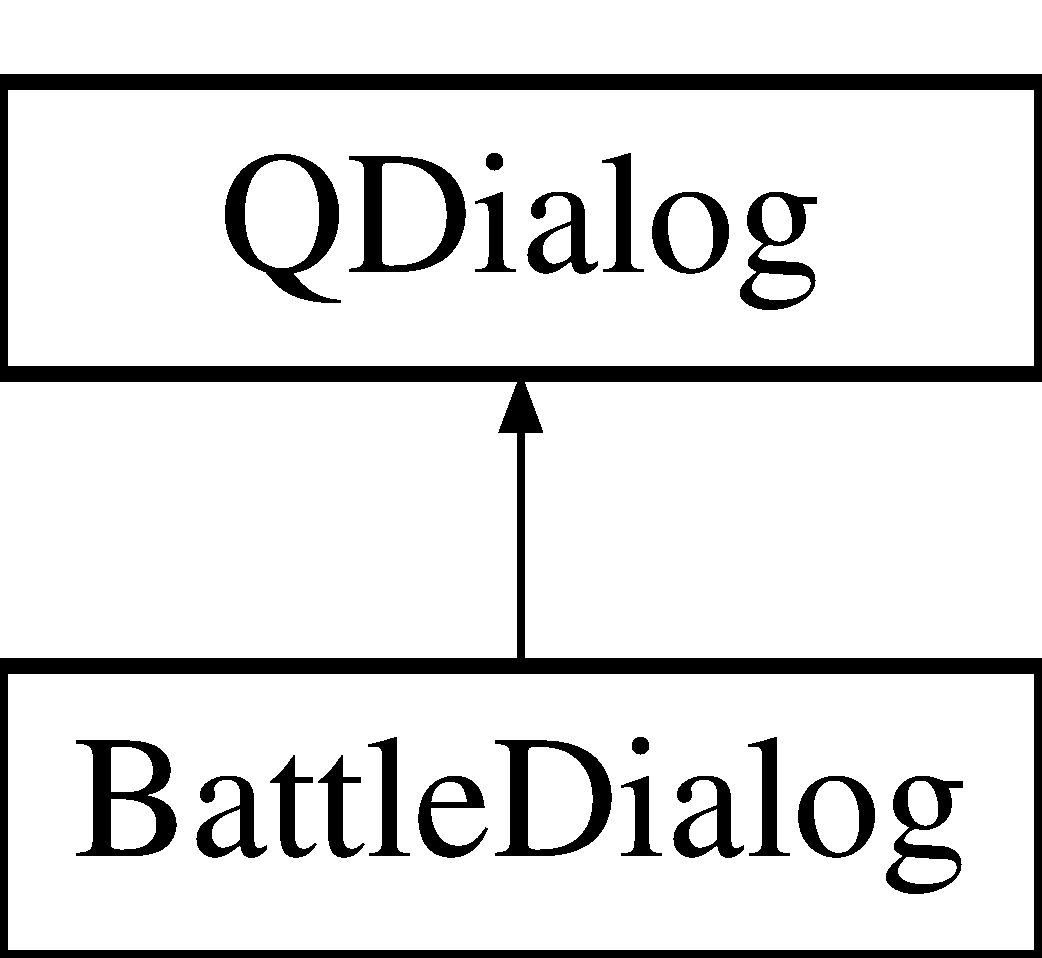
\includegraphics[height=2.000000cm]{class_battle_dialog}
\end{center}
\end{figure}
\subsection*{Public Member Functions}
\begin{DoxyCompactItemize}
\item 
\mbox{\Hypertarget{class_battle_dialog_af613b3d81895f3907122da94a3033b94}\label{class_battle_dialog_af613b3d81895f3907122da94a3033b94}} 
{\bfseries Battle\+Dialog} (Q\+Widget $\ast$parent=0)
\end{DoxyCompactItemize}


The documentation for this class was generated from the following files\+:\begin{DoxyCompactItemize}
\item 
battledialog.\+h\item 
battledialog.\+cpp\end{DoxyCompactItemize}

\hypertarget{class_ui_1_1_battle_dialog}{}\section{Ui\+:\+:Battle\+Dialog Class Reference}
\label{class_ui_1_1_battle_dialog}\index{Ui\+::\+Battle\+Dialog@{Ui\+::\+Battle\+Dialog}}
Inheritance diagram for Ui\+:\+:Battle\+Dialog\+:\begin{figure}[H]
\begin{center}
\leavevmode
\includegraphics[height=2.000000cm]{class_ui_1_1_battle_dialog}
\end{center}
\end{figure}
\subsection*{Additional Inherited Members}


The documentation for this class was generated from the following file\+:\begin{DoxyCompactItemize}
\item 
ui\+\_\+battledialog.\+h\end{DoxyCompactItemize}

\hypertarget{class_card}{}\section{Card Class Reference}
\label{class_card}\index{Card@{Card}}
Inheritance diagram for Card\+:\begin{figure}[H]
\begin{center}
\leavevmode
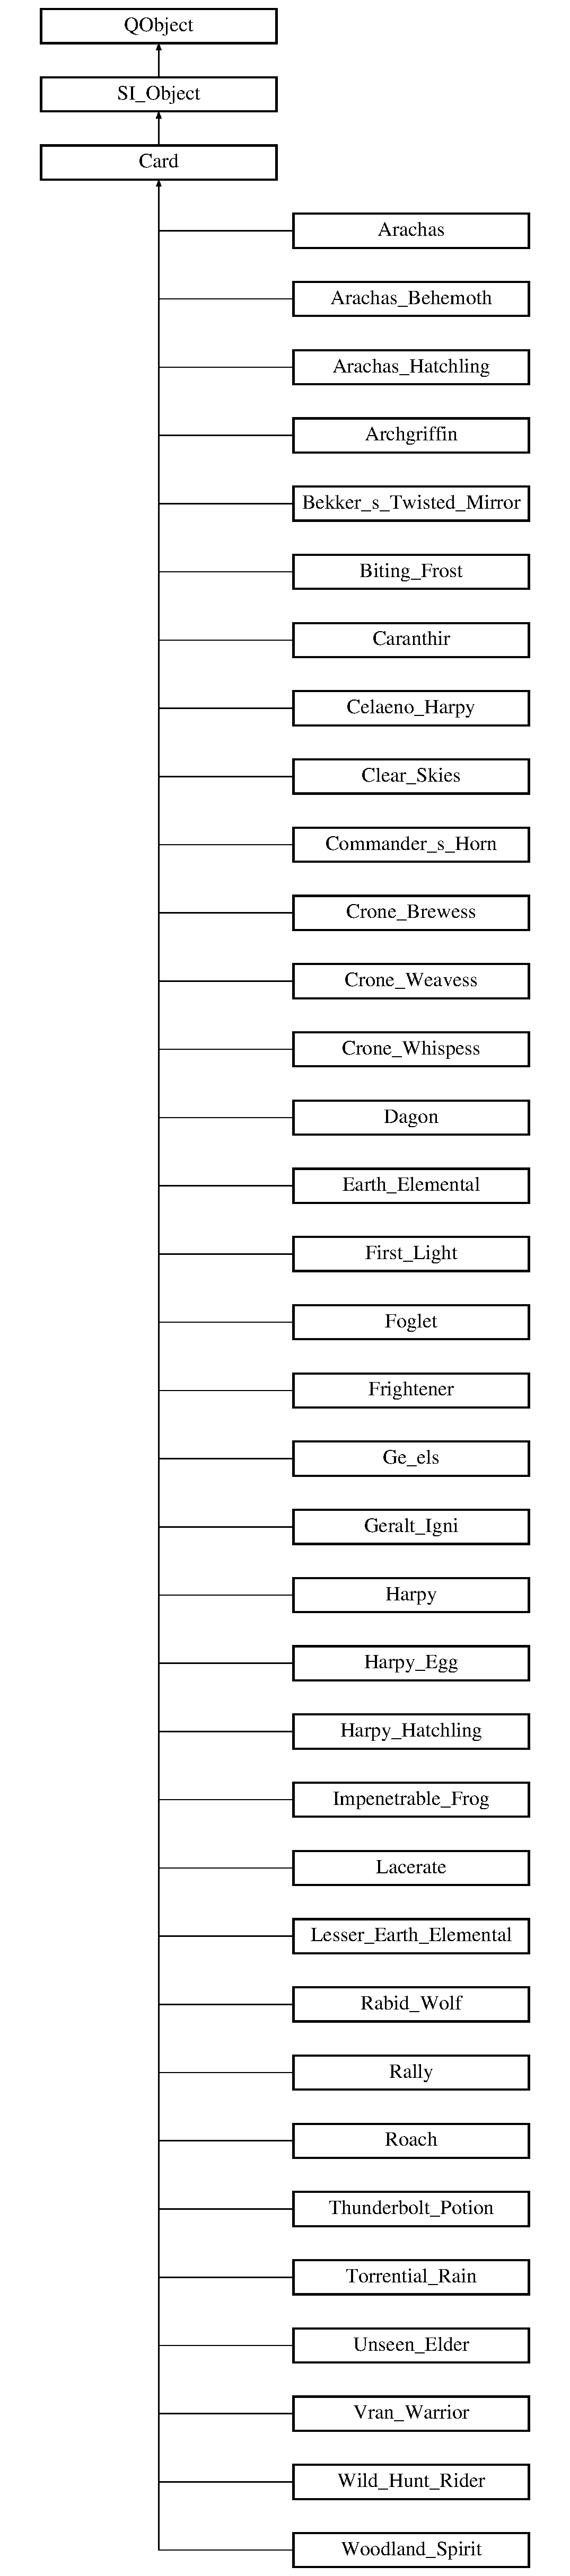
\includegraphics[height=3.000000cm]{class_card}
\end{center}
\end{figure}
\subsection*{Public Slots}
\begin{DoxyCompactItemize}
\item 
\mbox{\Hypertarget{class_card_a75b65d674f42ab381ebd53c8c156e31d}\label{class_card_a75b65d674f42ab381ebd53c8c156e31d}} 
virtual void {\bfseries \+\_\+played\+\_\+} (\hyperlink{class_card_set}{Row} $\ast$, int, \hyperlink{class_s_i___object}{S\+I\+\_\+\+Object} $\ast$, S\+I\+\_\+\+String)
\item 
\mbox{\Hypertarget{class_card_a353ffa2805c988fde980a67e6745a9bc}\label{class_card_a353ffa2805c988fde980a67e6745a9bc}} 
virtual void {\bfseries \+\_\+dameged\+\_\+} (int, \hyperlink{class_s_i___object}{S\+I\+\_\+\+Object} $\ast$, S\+I\+\_\+\+String)
\item 
\mbox{\Hypertarget{class_card_a8a98eab9a7a5a4c50a1e336751b709ed}\label{class_card_a8a98eab9a7a5a4c50a1e336751b709ed}} 
virtual void {\bfseries \+\_\+destroyed\+\_\+} (\hyperlink{class_s_i___object}{S\+I\+\_\+\+Object} $\ast$, S\+I\+\_\+\+String)
\item 
\mbox{\Hypertarget{class_card_ac722ae5b2fe10cbbd61a7970a44a9b69}\label{class_card_ac722ae5b2fe10cbbd61a7970a44a9b69}} 
virtual void {\bfseries \+\_\+exiled\+\_\+} (\hyperlink{class_s_i___object}{S\+I\+\_\+\+Object} $\ast$, S\+I\+\_\+\+String)
\item 
\mbox{\Hypertarget{class_card_a4da0f5dd31f60daac0549aa69ade4ba0}\label{class_card_a4da0f5dd31f60daac0549aa69ade4ba0}} 
virtual void {\bfseries \+\_\+drawed\+\_\+} (\hyperlink{class_s_i___object}{S\+I\+\_\+\+Object} $\ast$, S\+I\+\_\+\+String)
\item 
\mbox{\Hypertarget{class_card_a19a97de51f7a18f8204b86667960b78b}\label{class_card_a19a97de51f7a18f8204b86667960b78b}} 
virtual void {\bfseries \+\_\+boosted\+\_\+} (int, \hyperlink{class_s_i___object}{S\+I\+\_\+\+Object} $\ast$, S\+I\+\_\+\+String)
\item 
\mbox{\Hypertarget{class_card_acbccbb53af9bb57aec878c6a089d976f}\label{class_card_acbccbb53af9bb57aec878c6a089d976f}} 
virtual void {\bfseries \+\_\+adjust\+Base\+Power\+\_\+} (int, int, \hyperlink{class_s_i___object}{S\+I\+\_\+\+Object} $\ast$, S\+I\+\_\+\+String)
\item 
\mbox{\Hypertarget{class_card_aa3038c21b3d53d2076654d37fcc585e5}\label{class_card_aa3038c21b3d53d2076654d37fcc585e5}} 
virtual void {\bfseries \+\_\+adjust\+Boost\+Power\+\_\+} (int, int, \hyperlink{class_s_i___object}{S\+I\+\_\+\+Object} $\ast$, S\+I\+\_\+\+String)
\item 
\mbox{\Hypertarget{class_card_a6ce9a7fb0dc2b38981ccab8216a5588a}\label{class_card_a6ce9a7fb0dc2b38981ccab8216a5588a}} 
virtual void {\bfseries \+\_\+adjust\+Armor\+\_\+} (int, int, \hyperlink{class_s_i___object}{S\+I\+\_\+\+Object} $\ast$, S\+I\+\_\+\+String)
\item 
\mbox{\Hypertarget{class_card_a67ffdf0e225ded605fa32ef3d6890a2d}\label{class_card_a67ffdf0e225ded605fa32ef3d6890a2d}} 
virtual void {\bfseries \+\_\+strengthened\+\_\+} (int, \hyperlink{class_s_i___object}{S\+I\+\_\+\+Object} $\ast$, S\+I\+\_\+\+String)
\item 
\mbox{\Hypertarget{class_card_a63ec79b62dd31b7f79f3819267e21d38}\label{class_card_a63ec79b62dd31b7f79f3819267e21d38}} 
virtual void {\bfseries \+\_\+weakened\+\_\+} (int, \hyperlink{class_s_i___object}{S\+I\+\_\+\+Object} $\ast$, S\+I\+\_\+\+String)
\item 
\mbox{\Hypertarget{class_card_a2dc7770bef7278725955080a4e3d2a04}\label{class_card_a2dc7770bef7278725955080a4e3d2a04}} 
virtual void {\bfseries \+\_\+reseted\+\_\+} (\hyperlink{class_s_i___object}{S\+I\+\_\+\+Object} $\ast$, S\+I\+\_\+\+String)
\item 
\mbox{\Hypertarget{class_card_a327252206ff2240215bc387d943b641c}\label{class_card_a327252206ff2240215bc387d943b641c}} 
virtual void {\bfseries \+\_\+adjust\+Place\+\_\+} (\hyperlink{class_card_set}{Card\+Set} $\ast$, int, \hyperlink{class_card_set}{Card\+Set} $\ast$, int, \hyperlink{class_s_i___object}{S\+I\+\_\+\+Object} $\ast$, S\+I\+\_\+\+String)
\item 
\mbox{\Hypertarget{class_card_ade9c389ec3c13bbc84cc23320d787665}\label{class_card_ade9c389ec3c13bbc84cc23320d787665}} 
virtual void {\bfseries \+\_\+consumed\+\_\+} (\hyperlink{class_card}{Card} $\ast$, \hyperlink{class_s_i___object}{S\+I\+\_\+\+Object} $\ast$, S\+I\+\_\+\+String)
\item 
\mbox{\Hypertarget{class_card_a46b1bf27235cf35ecea38eca05ac6756}\label{class_card_a46b1bf27235cf35ecea38eca05ac6756}} 
virtual void {\bfseries \+\_\+consume\+\_\+} (\hyperlink{class_card}{Card} $\ast$, \hyperlink{class_s_i___object}{S\+I\+\_\+\+Object} $\ast$, S\+I\+\_\+\+String)
\end{DoxyCompactItemize}
\subsection*{Signals}
\begin{DoxyCompactItemize}
\item 
\mbox{\Hypertarget{class_card_a9df468ae60047dea8dcf7a71fb4eb071}\label{class_card_a9df468ae60047dea8dcf7a71fb4eb071}} 
void {\bfseries played\+\_\+} (\hyperlink{class_card_set}{Row} $\ast$, int, \hyperlink{class_s_i___object}{S\+I\+\_\+\+Object} $\ast$, S\+I\+\_\+\+String)
\item 
\mbox{\Hypertarget{class_card_aa1882f8263bd74313148a0010206a36a}\label{class_card_aa1882f8263bd74313148a0010206a36a}} 
void {\bfseries dameged\+\_\+} (int, \hyperlink{class_s_i___object}{S\+I\+\_\+\+Object} $\ast$, S\+I\+\_\+\+String)
\item 
\mbox{\Hypertarget{class_card_adbf89377f717c353eb26e9a6fc9130e4}\label{class_card_adbf89377f717c353eb26e9a6fc9130e4}} 
void {\bfseries destroyed\+\_\+} (\hyperlink{class_s_i___object}{S\+I\+\_\+\+Object} $\ast$, S\+I\+\_\+\+String)
\item 
\mbox{\Hypertarget{class_card_af74e10d19deffaedf6d40e916b38a601}\label{class_card_af74e10d19deffaedf6d40e916b38a601}} 
void {\bfseries exiled\+\_\+} (\hyperlink{class_s_i___object}{S\+I\+\_\+\+Object} $\ast$, S\+I\+\_\+\+String)
\item 
\mbox{\Hypertarget{class_card_a0175ac76e02db0997d285212eeed3423}\label{class_card_a0175ac76e02db0997d285212eeed3423}} 
void {\bfseries drawed\+\_\+} (\hyperlink{class_s_i___object}{S\+I\+\_\+\+Object} $\ast$, S\+I\+\_\+\+String)
\item 
\mbox{\Hypertarget{class_card_afbafa9d69894f687ba7a2f7b0cd8a5dc}\label{class_card_afbafa9d69894f687ba7a2f7b0cd8a5dc}} 
void {\bfseries boosted\+\_\+} (int, \hyperlink{class_s_i___object}{S\+I\+\_\+\+Object} $\ast$, S\+I\+\_\+\+String)
\item 
\mbox{\Hypertarget{class_card_ac38dfd022350292672a23f5dbe690a4c}\label{class_card_ac38dfd022350292672a23f5dbe690a4c}} 
void {\bfseries adjust\+Base\+Power\+\_\+} (int, int, \hyperlink{class_s_i___object}{S\+I\+\_\+\+Object} $\ast$, S\+I\+\_\+\+String)
\item 
\mbox{\Hypertarget{class_card_ac3b4d7d244400105782caea99940c4d8}\label{class_card_ac3b4d7d244400105782caea99940c4d8}} 
void {\bfseries adjust\+Boost\+Power\+\_\+} (int, int, \hyperlink{class_s_i___object}{S\+I\+\_\+\+Object} $\ast$, S\+I\+\_\+\+String)
\item 
\mbox{\Hypertarget{class_card_a3bf57c66d92a7c40d450b2072eb5c643}\label{class_card_a3bf57c66d92a7c40d450b2072eb5c643}} 
void {\bfseries adjust\+Armor\+\_\+} (int, int, \hyperlink{class_s_i___object}{S\+I\+\_\+\+Object} $\ast$, S\+I\+\_\+\+String)
\item 
\mbox{\Hypertarget{class_card_a8842b16cfab0bd061cbd7962b54bf69d}\label{class_card_a8842b16cfab0bd061cbd7962b54bf69d}} 
void {\bfseries strengthened\+\_\+} (int, \hyperlink{class_s_i___object}{S\+I\+\_\+\+Object} $\ast$, S\+I\+\_\+\+String)
\item 
\mbox{\Hypertarget{class_card_a6df9b23b65116dbc8e4b76526030fe2c}\label{class_card_a6df9b23b65116dbc8e4b76526030fe2c}} 
void {\bfseries weakened\+\_\+} (int, \hyperlink{class_s_i___object}{S\+I\+\_\+\+Object} $\ast$, S\+I\+\_\+\+String)
\item 
\mbox{\Hypertarget{class_card_a2a94d6d15649199fae7a972f436fc3f3}\label{class_card_a2a94d6d15649199fae7a972f436fc3f3}} 
void {\bfseries reseted\+\_\+} (\hyperlink{class_s_i___object}{S\+I\+\_\+\+Object} $\ast$, S\+I\+\_\+\+String)
\item 
\mbox{\Hypertarget{class_card_a5d230a2e76a0b74ddc3f848b5f0fdc82}\label{class_card_a5d230a2e76a0b74ddc3f848b5f0fdc82}} 
void {\bfseries adjust\+Place\+\_\+} (\hyperlink{class_card_set}{Card\+Set} $\ast$, int, \hyperlink{class_card_set}{Card\+Set} $\ast$, int, \hyperlink{class_s_i___object}{S\+I\+\_\+\+Object} $\ast$, S\+I\+\_\+\+String)
\item 
\mbox{\Hypertarget{class_card_ade61baff01ef01fd93a6cdcd18e1c1bb}\label{class_card_ade61baff01ef01fd93a6cdcd18e1c1bb}} 
void {\bfseries consume\+\_\+} (\hyperlink{class_card}{Card} $\ast$, \hyperlink{class_s_i___object}{S\+I\+\_\+\+Object} $\ast$, S\+I\+\_\+\+String)
\item 
\mbox{\Hypertarget{class_card_ab521eee2c82fdef858eb6cf33b396e31}\label{class_card_ab521eee2c82fdef858eb6cf33b396e31}} 
void {\bfseries consumed\+\_\+} (\hyperlink{class_card}{Card} $\ast$, \hyperlink{class_s_i___object}{S\+I\+\_\+\+Object} $\ast$, S\+I\+\_\+\+String)
\end{DoxyCompactItemize}
\subsection*{Public Member Functions}
\begin{DoxyCompactItemize}
\item 
\mbox{\Hypertarget{class_card_a6028479328172961db1bf1a508ed09b0}\label{class_card_a6028479328172961db1bf1a508ed09b0}} 
{\bfseries Card} (Q\+Object $\ast$parent=0)
\item 
\mbox{\Hypertarget{class_card_a3797acfaee3be9d91b3c0ebc09490b56}\label{class_card_a3797acfaee3be9d91b3c0ebc09490b56}} 
{\bfseries Card} (const \hyperlink{class_card}{Card} \&tcard)
\item 
\mbox{\Hypertarget{class_card_a27001cb04a123c389457e599387e9ea8}\label{class_card_a27001cb04a123c389457e599387e9ea8}} 
bool {\bfseries \+\_\+\+\_\+init\+Info} ()
\item 
\mbox{\Hypertarget{class_card_a1ab2585666a2197ca28a5f4de71aecb8}\label{class_card_a1ab2585666a2197ca28a5f4de71aecb8}} 
void {\bfseries \+\_\+\+\_\+read\+Info} (Q\+Text\+Stream \&)
\item 
\mbox{\Hypertarget{class_card_a33d357ac1f0043989f87c0c24d3e24e9}\label{class_card_a33d357ac1f0043989f87c0c24d3e24e9}} 
void {\bfseries \+\_\+\+\_\+init} ()
\item 
\mbox{\Hypertarget{class_card_a77f2d72697f3d2cd7145d72c397894fc}\label{class_card_a77f2d72697f3d2cd7145d72c397894fc}} 
void {\bfseries call\+Function} (S\+I\+\_\+\+String)
\item 
\mbox{\Hypertarget{class_card_a8594374030d81e2ff7810df6fc64b63e}\label{class_card_a8594374030d81e2ff7810df6fc64b63e}} 
\hyperlink{class_card_set}{Card\+Set} $\ast$ {\bfseries get\+Place} () const
\item 
\mbox{\Hypertarget{class_card_ae4752ed5bf120afc48e9fd65ea6dab52}\label{class_card_ae4752ed5bf120afc48e9fd65ea6dab52}} 
int {\bfseries get\+Order} () const
\item 
\mbox{\Hypertarget{class_card_a660219c0fc2677abea4f8dfb2f8d3449}\label{class_card_a660219c0fc2677abea4f8dfb2f8d3449}} 
void {\bfseries set\+Place} (\hyperlink{class_card_set}{Card\+Set} $\ast$, int)
\item 
\mbox{\Hypertarget{class_card_a6c6b39f3b6c64d5775e172dcfaefdf89}\label{class_card_a6c6b39f3b6c64d5775e172dcfaefdf89}} 
void {\bfseries get\+Position} (int \&, int \&)
\item 
\mbox{\Hypertarget{class_card_a9ac3fd6811dfbb5fef7ab507c5ae52e5}\label{class_card_a9ac3fd6811dfbb5fef7ab507c5ae52e5}} 
void {\bfseries destroy} ()
\item 
\mbox{\Hypertarget{class_card_ad89cc3cf4c2afb10381655bf5940dec6}\label{class_card_ad89cc3cf4c2afb10381655bf5940dec6}} 
void {\bfseries set\+Game} (\hyperlink{class_game}{Game} $\ast$)
\item 
\mbox{\Hypertarget{class_card_afda7a2a346514b795d979494c68f5e15}\label{class_card_afda7a2a346514b795d979494c68f5e15}} 
void {\bfseries setup} (int, \hyperlink{class_game}{Game} $\ast$)
\item 
\mbox{\Hypertarget{class_card_aaf4b38dccc9e9d2cec7db8e1a8fa2efc}\label{class_card_aaf4b38dccc9e9d2cec7db8e1a8fa2efc}} 
virtual void {\bfseries \+\_\+\+\_\+do\+Connect} ()
\item 
\mbox{\Hypertarget{class_card_a8a9fdf9ebc85896727159f11886b0bea}\label{class_card_a8a9fdf9ebc85896727159f11886b0bea}} 
void {\bfseries \+\_\+\+\_\+\+\_\+print} ()
\end{DoxyCompactItemize}
\subsection*{Static Public Member Functions}
\begin{DoxyCompactItemize}
\item 
\mbox{\Hypertarget{class_card_abce1758283c642a8465655e855acc763}\label{class_card_abce1758283c642a8465655e855acc763}} 
static \hyperlink{class_card}{Card} $\ast$ {\bfseries factory} (\hyperlink{class_game}{Game} $\ast$, S\+I\+\_\+\+String)
\end{DoxyCompactItemize}
\subsection*{Public Attributes}
\begin{DoxyCompactItemize}
\item 
\mbox{\Hypertarget{class_card_aae5c395ef6504102afea9bbf68a7bf73}\label{class_card_aae5c395ef6504102afea9bbf68a7bf73}} 
\hyperlink{class_card_set}{Card\+Set} $\ast$ {\bfseries place}
\item 
\mbox{\Hypertarget{class_card_a525e165be1a96a9c76b6b3959d8f67f6}\label{class_card_a525e165be1a96a9c76b6b3959d8f67f6}} 
\hyperlink{class_game}{Game} $\ast$ {\bfseries game}
\item 
\mbox{\Hypertarget{class_card_ae6fb6f495bba4d639696f934b495c15f}\label{class_card_ae6fb6f495bba4d639696f934b495c15f}} 
int {\bfseries id}
\item 
\mbox{\Hypertarget{class_card_a79a46e893cf63f7aa582800bea836eb3}\label{class_card_a79a46e893cf63f7aa582800bea836eb3}} 
int {\bfseries cid}
\item 
\mbox{\Hypertarget{class_card_a30038db90de96f57756bb88d1fbfb05f}\label{class_card_a30038db90de96f57756bb88d1fbfb05f}} 
\hyperlink{class_card_widget}{Card\+Widget} $\ast$ {\bfseries pwidget}
\end{DoxyCompactItemize}
\subsection*{Static Public Attributes}
\begin{DoxyCompactItemize}
\item 
\mbox{\Hypertarget{class_card_a02f1c740facc2458b2199a1802263147}\label{class_card_a02f1c740facc2458b2199a1802263147}} 
static S\+I\+\_\+\+String {\bfseries card\+Dir} =\char`\"{}\+:/card/src/card/\char`\"{}
\end{DoxyCompactItemize}
\subsection*{Friends}
\begin{DoxyCompactItemize}
\item 
\mbox{\Hypertarget{class_card_aaec47a26a3c11c1debd3ed922b69cbd2}\label{class_card_aaec47a26a3c11c1debd3ed922b69cbd2}} 
class {\bfseries Field}
\end{DoxyCompactItemize}


The documentation for this class was generated from the following files\+:\begin{DoxyCompactItemize}
\item 
card.\+h\item 
card.\+cpp\end{DoxyCompactItemize}

\hypertarget{class_card_set}{}\section{Card\+Set Class Reference}
\label{class_card_set}\index{Card\+Set@{Card\+Set}}
Inheritance diagram for Card\+Set\+:\begin{figure}[H]
\begin{center}
\leavevmode
\includegraphics[height=3.000000cm]{class_card_set}
\end{center}
\end{figure}
\subsection*{Public Slots}
\begin{DoxyCompactItemize}
\item 
\mbox{\Hypertarget{class_card_set_aceb4ca4e4afc86a9e023d9fe8d4e4779}\label{class_card_set_aceb4ca4e4afc86a9e023d9fe8d4e4779}} 
void {\bfseries clear} ()
\item 
\mbox{\Hypertarget{class_card_set_ae0800ef1090156cc46b19fec949fe91f}\label{class_card_set_ae0800ef1090156cc46b19fec949fe91f}} 
void {\bfseries re\+Order} ()
\item 
\mbox{\Hypertarget{class_card_set_a8b7912316916ea6c69f151ecfdbcddb9}\label{class_card_set_a8b7912316916ea6c69f151ecfdbcddb9}} 
void {\bfseries erase} (\hyperlink{class_card}{Card} \&)
\item 
\mbox{\Hypertarget{class_card_set_a8dc3d979e356f0d97ebea17a1b8fc539}\label{class_card_set_a8dc3d979e356f0d97ebea17a1b8fc539}} 
void {\bfseries erase} (\hyperlink{class_card}{Card} $\ast$)
\item 
\mbox{\Hypertarget{class_card_set_a5e61777b1d1eb2ca933ef5c16eb0e945}\label{class_card_set_a5e61777b1d1eb2ca933ef5c16eb0e945}} 
void {\bfseries ins} (\hyperlink{class_card}{Card} $\ast$, int)
\item 
\mbox{\Hypertarget{class_card_set_ae2da9ca0de5572e3d045b61233b3c134}\label{class_card_set_ae2da9ca0de5572e3d045b61233b3c134}} 
list$<$ \hyperlink{class_card}{Card} $\ast$ $>$\+::iterator {\bfseries \+\_\+get\+Iterator} (int)
\item 
\mbox{\Hypertarget{class_card_set_a8fbebc315fd5f9fd62e3f0ae081883e2}\label{class_card_set_a8fbebc315fd5f9fd62e3f0ae081883e2}} 
list$<$ \hyperlink{class_card}{Card} $\ast$ $>$\+::iterator {\bfseries \+\_\+get\+Iterator} (\hyperlink{class_card}{Card} $\ast$)
\end{DoxyCompactItemize}
\subsection*{Public Member Functions}
\begin{DoxyCompactItemize}
\item 
\mbox{\Hypertarget{class_card_set_ab71f7d1a3ff84bbe38a15a9f3763cc51}\label{class_card_set_ab71f7d1a3ff84bbe38a15a9f3763cc51}} 
{\bfseries Card\+Set} (Q\+Object $\ast$parent=0)
\item 
\mbox{\Hypertarget{class_card_set_aa1bc47338af30630e2bf531efbe0cf56}\label{class_card_set_aa1bc47338af30630e2bf531efbe0cf56}} 
\hyperlink{class_card}{Card} $\ast$ {\bfseries at\+Index} (int)
\item 
\mbox{\Hypertarget{class_card_set_aaeac4f9e1a5560457653f42416721459}\label{class_card_set_aaeac4f9e1a5560457653f42416721459}} 
bool {\bfseries check\+Card} (\hyperlink{class_card}{Card} $\ast$)
\item 
\mbox{\Hypertarget{class_card_set_a5869ddf6190c03ce3bc5ce77139708e4}\label{class_card_set_a5869ddf6190c03ce3bc5ce77139708e4}} 
void {\bfseries \+\_\+\+\_\+change\+Score} (int)
\item 
\mbox{\Hypertarget{class_card_set_ab025d30be863978e10536c97874fbbe5}\label{class_card_set_ab025d30be863978e10536c97874fbbe5}} 
void {\bfseries \+\_\+\+\_\+\+\_\+print} ()
\end{DoxyCompactItemize}
\subsection*{Public Attributes}
\begin{DoxyCompactItemize}
\item 
\mbox{\Hypertarget{class_card_set_a1edd225de05154f8feafc2afab4dd22b}\label{class_card_set_a1edd225de05154f8feafc2afab4dd22b}} 
list$<$ \hyperlink{class_card}{Card} $\ast$ $>$ {\bfseries card\+Set}
\item 
\mbox{\Hypertarget{class_card_set_ad216ddc2e60b7e83c8bd3ab35d22cde0}\label{class_card_set_ad216ddc2e60b7e83c8bd3ab35d22cde0}} 
\hyperlink{class_card_set}{Card\+Set} $\ast$ {\bfseries fath}
\item 
\mbox{\Hypertarget{class_card_set_a04ee7f62a134fee4c15199eec78614d8}\label{class_card_set_a04ee7f62a134fee4c15199eec78614d8}} 
\hyperlink{class_weather}{Weather} $\ast$ {\bfseries weather}
\item 
\mbox{\Hypertarget{class_card_set_aa46653ada53e7a80af71309a8a93cc3e}\label{class_card_set_aa46653ada53e7a80af71309a8a93cc3e}} 
int {\bfseries score}
\end{DoxyCompactItemize}
\subsection*{Additional Inherited Members}


The documentation for this class was generated from the following files\+:\begin{DoxyCompactItemize}
\item 
cardset.\+h\item 
cardset.\+cpp\end{DoxyCompactItemize}

\hypertarget{class_card_set_widget}{}\section{Card\+Set\+Widget Class Reference}
\label{class_card_set_widget}\index{Card\+Set\+Widget@{Card\+Set\+Widget}}
Inheritance diagram for Card\+Set\+Widget\+:\begin{figure}[H]
\begin{center}
\leavevmode
\includegraphics[height=2.000000cm]{class_card_set_widget}
\end{center}
\end{figure}
\subsection*{Public Member Functions}
\begin{DoxyCompactItemize}
\item 
\mbox{\Hypertarget{class_card_set_widget_a81a41cbdce77cfca7dd118ae0cf0b3fe}\label{class_card_set_widget_a81a41cbdce77cfca7dd118ae0cf0b3fe}} 
{\bfseries Card\+Set\+Widget} (\hyperlink{class_card_set}{Card\+Set} $\ast$tpcard\+Set, Q\+Widget $\ast$parent=0)
\item 
\mbox{\Hypertarget{class_card_set_widget_a565197943c3919bb14117133d351bc67}\label{class_card_set_widget_a565197943c3919bb14117133d351bc67}} 
void {\bfseries \+\_\+update} ()
\end{DoxyCompactItemize}
\subsection*{Public Attributes}
\begin{DoxyCompactItemize}
\item 
\mbox{\Hypertarget{class_card_set_widget_aa21084283c057497f40de8a19ba03c89}\label{class_card_set_widget_aa21084283c057497f40de8a19ba03c89}} 
Q\+Grid\+Layout $\ast$ {\bfseries w\+\_\+mainlayout}
\item 
\mbox{\Hypertarget{class_card_set_widget_adedb07d0aef53fe5e02843df01920cd3}\label{class_card_set_widget_adedb07d0aef53fe5e02843df01920cd3}} 
Q\+Grid\+Layout $\ast$ {\bfseries w\+\_\+glayout}
\item 
\mbox{\Hypertarget{class_card_set_widget_aafc82808936be8d82723ad11ec5fd55c}\label{class_card_set_widget_aafc82808936be8d82723ad11ec5fd55c}} 
Q\+Widget $\ast$ {\bfseries w\+\_\+mainwidget}
\item 
\mbox{\Hypertarget{class_card_set_widget_abe9de3a3f7ef9d7010fad6a7eac862b7}\label{class_card_set_widget_abe9de3a3f7ef9d7010fad6a7eac862b7}} 
\hyperlink{class_card_set}{Card\+Set} $\ast$ {\bfseries pcard\+Set}
\end{DoxyCompactItemize}


The documentation for this class was generated from the following files\+:\begin{DoxyCompactItemize}
\item 
cardsetwidget.\+h\item 
cardsetwidget.\+cpp\end{DoxyCompactItemize}

\hypertarget{class_ui_1_1_card_set_widget}{}\section{Ui\+:\+:Card\+Set\+Widget Class Reference}
\label{class_ui_1_1_card_set_widget}\index{Ui\+::\+Card\+Set\+Widget@{Ui\+::\+Card\+Set\+Widget}}
Inheritance diagram for Ui\+:\+:Card\+Set\+Widget\+:\begin{figure}[H]
\begin{center}
\leavevmode
\includegraphics[height=2.000000cm]{class_ui_1_1_card_set_widget}
\end{center}
\end{figure}
\subsection*{Additional Inherited Members}


The documentation for this class was generated from the following file\+:\begin{DoxyCompactItemize}
\item 
ui\+\_\+cardsetwidget.\+h\end{DoxyCompactItemize}

\hypertarget{class_ui_1_1_card_widget}{}\section{Ui\+:\+:Card\+Widget Class Reference}
\label{class_ui_1_1_card_widget}\index{Ui\+::\+Card\+Widget@{Ui\+::\+Card\+Widget}}
Inheritance diagram for Ui\+:\+:Card\+Widget\+:\begin{figure}[H]
\begin{center}
\leavevmode
\includegraphics[height=2.000000cm]{class_ui_1_1_card_widget}
\end{center}
\end{figure}
\subsection*{Additional Inherited Members}


The documentation for this class was generated from the following file\+:\begin{DoxyCompactItemize}
\item 
ui\+\_\+cardwidget.\+h\end{DoxyCompactItemize}

\hypertarget{class_card_widget}{}\section{Card\+Widget Class Reference}
\label{class_card_widget}\index{Card\+Widget@{Card\+Widget}}
Inheritance diagram for Card\+Widget\+:\begin{figure}[H]
\begin{center}
\leavevmode
\includegraphics[height=2.000000cm]{class_card_widget}
\end{center}
\end{figure}
\subsection*{Public Slots}
\begin{DoxyCompactItemize}
\item 
\mbox{\Hypertarget{class_card_widget_adbe8215dd0c765e654e25ba140753bfd}\label{class_card_widget_adbe8215dd0c765e654e25ba140753bfd}} 
void {\bfseries set\+Info\+Label} ()
\end{DoxyCompactItemize}
\subsection*{Public Member Functions}
\begin{DoxyCompactItemize}
\item 
\mbox{\Hypertarget{class_card_widget_a2c634d21182039e586d62709f6e1d49b}\label{class_card_widget_a2c634d21182039e586d62709f6e1d49b}} 
{\bfseries Card\+Widget} (\hyperlink{class_card}{Card} $\ast$, Q\+Widget $\ast$parent=0)
\item 
\mbox{\Hypertarget{class_card_widget_a768a4290ec339ddccc6e236f72fce14f}\label{class_card_widget_a768a4290ec339ddccc6e236f72fce14f}} 
void {\bfseries set\+Enabled} (bool)
\item 
\mbox{\Hypertarget{class_card_widget_ab1b658a6f432c2061029748198ef3e24}\label{class_card_widget_ab1b658a6f432c2061029748198ef3e24}} 
void {\bfseries set\+Name} (S\+I\+\_\+\+String)
\item 
\mbox{\Hypertarget{class_card_widget_aff538dc64ec9268b0e5ffabc17014f03}\label{class_card_widget_aff538dc64ec9268b0e5ffabc17014f03}} 
void {\bfseries set\+Power} (int)
\end{DoxyCompactItemize}
\subsection*{Public Attributes}
\begin{DoxyCompactItemize}
\item 
\mbox{\Hypertarget{class_card_widget_a8466130e2bf6f2db76bf6c42061036c3}\label{class_card_widget_a8466130e2bf6f2db76bf6c42061036c3}} 
Q\+Push\+Button $\ast$ {\bfseries w\+\_\+picbutton}
\item 
\mbox{\Hypertarget{class_card_widget_a500a89ece7e911444b632b76786820b3}\label{class_card_widget_a500a89ece7e911444b632b76786820b3}} 
Q\+Grid\+Layout $\ast$ {\bfseries w\+\_\+glayout}
\item 
\mbox{\Hypertarget{class_card_widget_a47ebad10252a186182dddc8bb4a59314}\label{class_card_widget_a47ebad10252a186182dddc8bb4a59314}} 
Q\+Icon {\bfseries icon}
\item 
\mbox{\Hypertarget{class_card_widget_a39d4de66056548aba91ac9b1925ae191}\label{class_card_widget_a39d4de66056548aba91ac9b1925ae191}} 
\hyperlink{class_card}{Card} $\ast$ {\bfseries pcard}
\end{DoxyCompactItemize}
\subsection*{Static Public Attributes}
\begin{DoxyCompactItemize}
\item 
\mbox{\Hypertarget{class_card_widget_a9cc2464f7d43b18f6b5d5a4e2363edaa}\label{class_card_widget_a9cc2464f7d43b18f6b5d5a4e2363edaa}} 
static S\+I\+\_\+\+String {\bfseries img\+Dir} =\char`\"{}\+:/img/src/img/\char`\"{}
\end{DoxyCompactItemize}


The documentation for this class was generated from the following files\+:\begin{DoxyCompactItemize}
\item 
cardwidget.\+h\item 
cardwidget.\+cpp\end{DoxyCompactItemize}

\hypertarget{class_deck_builder}{}\section{Deck\+Builder Class Reference}
\label{class_deck_builder}\index{Deck\+Builder@{Deck\+Builder}}
Inheritance diagram for Deck\+Builder\+:\begin{figure}[H]
\begin{center}
\leavevmode
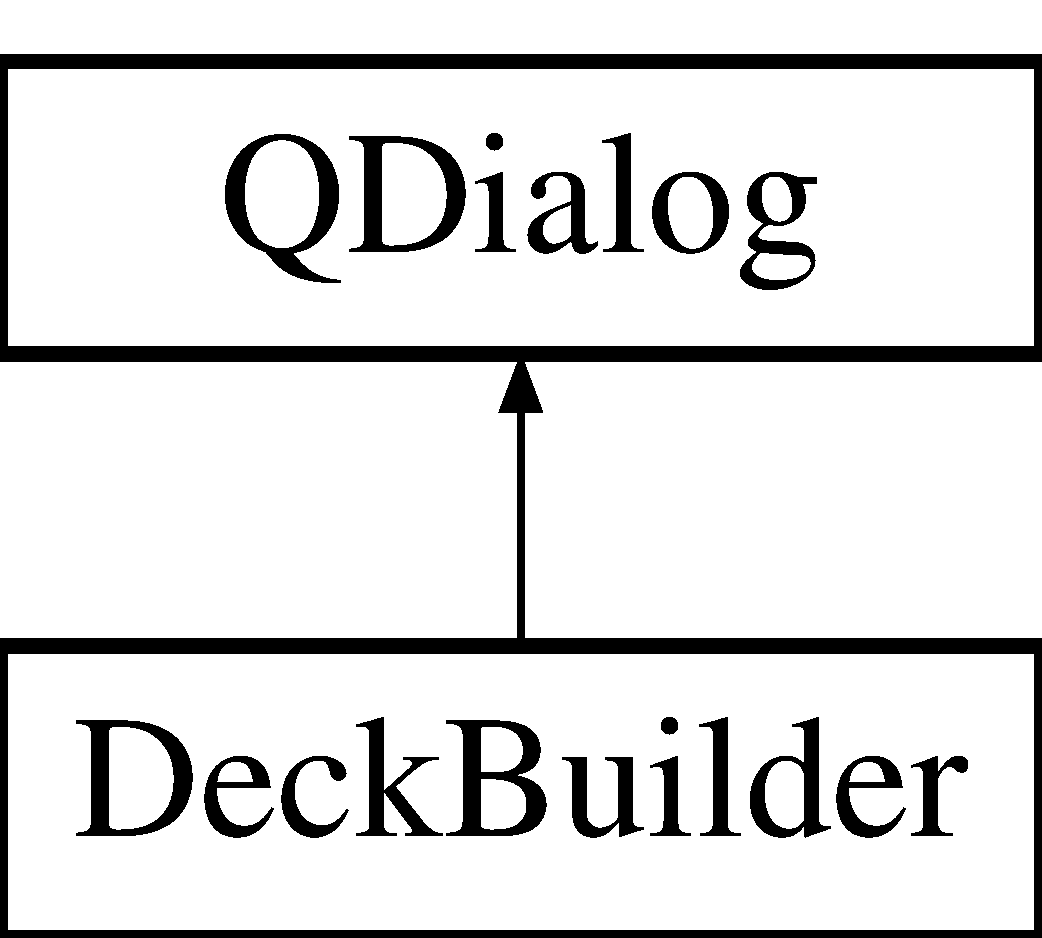
\includegraphics[height=2.000000cm]{class_deck_builder}
\end{center}
\end{figure}
\subsection*{Public Slots}
\begin{DoxyCompactItemize}
\item 
\mbox{\Hypertarget{class_deck_builder_a4f6b854f2e899978cfee769b60d4e383}\label{class_deck_builder_a4f6b854f2e899978cfee769b60d4e383}} 
void {\bfseries clicked} (int)
\item 
\mbox{\Hypertarget{class_deck_builder_a53e4027ab59c876b6c5b55be2b6abdf7}\label{class_deck_builder_a53e4027ab59c876b6c5b55be2b6abdf7}} 
void {\bfseries save} ()
\end{DoxyCompactItemize}
\subsection*{Public Member Functions}
\begin{DoxyCompactItemize}
\item 
\mbox{\Hypertarget{class_deck_builder_a27ddaae932ced02f22e26444ca391909}\label{class_deck_builder_a27ddaae932ced02f22e26444ca391909}} 
{\bfseries Deck\+Builder} (Q\+Widget $\ast$parent=0)
\end{DoxyCompactItemize}
\subsection*{Public Attributes}
\begin{DoxyCompactItemize}
\item 
\mbox{\Hypertarget{class_deck_builder_ae111e9bac35ec1c2140a50a6308c55ac}\label{class_deck_builder_ae111e9bac35ec1c2140a50a6308c55ac}} 
\hyperlink{class_game}{Game} $\ast$ {\bfseries game}
\item 
\mbox{\Hypertarget{class_deck_builder_a1d73429e77634d8a4698f9a86e1b9aed}\label{class_deck_builder_a1d73429e77634d8a4698f9a86e1b9aed}} 
Q\+Signal\+Mapper $\ast$ {\bfseries mapper}
\item 
\mbox{\Hypertarget{class_deck_builder_aa7d6acc263ed5f017189614d4650e2aa}\label{class_deck_builder_aa7d6acc263ed5f017189614d4650e2aa}} 
\hyperlink{class_card_set}{Card\+Set} $\ast$ {\bfseries view\+Place}
\end{DoxyCompactItemize}


The documentation for this class was generated from the following files\+:\begin{DoxyCompactItemize}
\item 
deckbuilder.\+h\item 
deckbuilder.\+cpp\end{DoxyCompactItemize}

\hypertarget{class_field}{}\section{Field Class Reference}
\label{class_field}\index{Field@{Field}}
Inheritance diagram for Field\+:\begin{figure}[H]
\begin{center}
\leavevmode
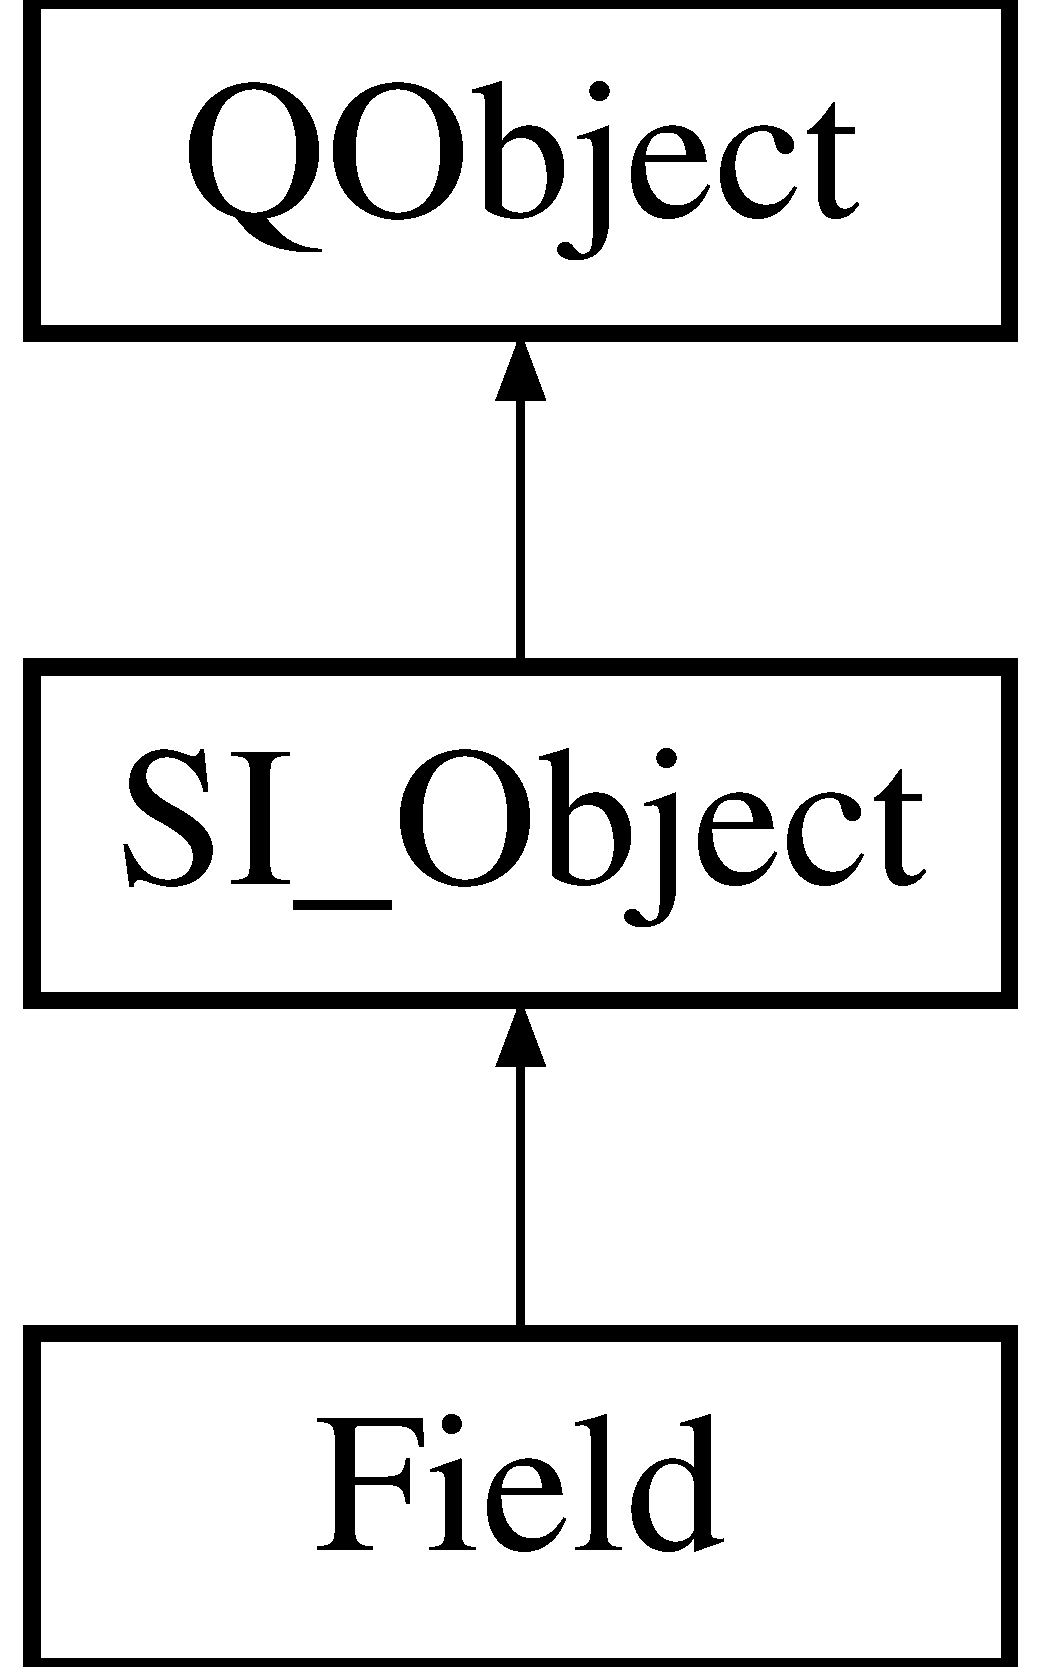
\includegraphics[height=3.000000cm]{class_field}
\end{center}
\end{figure}
\subsection*{Public Slots}
\begin{DoxyCompactItemize}
\item 
\mbox{\Hypertarget{class_field_ac37ae12cc1b0552829f69a9e643290b6}\label{class_field_ac37ae12cc1b0552829f69a9e643290b6}} 
void {\bfseries play\+Card} (\hyperlink{class_card}{Card} $\ast$, \hyperlink{class_card_set}{Row} $\ast$, int, \hyperlink{class_s_i___object}{S\+I\+\_\+\+Object} $\ast$, S\+I\+\_\+\+String)
\item 
\mbox{\Hypertarget{class_field_a6714bf36ca89295fbc8cbb67b40ecd66}\label{class_field_a6714bf36ca89295fbc8cbb67b40ecd66}} 
void {\bfseries revive\+Card} (\hyperlink{class_card}{Card} $\ast$, \hyperlink{class_card_set}{Row} $\ast$, int, \hyperlink{class_s_i___object}{S\+I\+\_\+\+Object} $\ast$, S\+I\+\_\+\+String)
\item 
\mbox{\Hypertarget{class_field_ab5b8e86a9652c2525c454b9a0c095787}\label{class_field_ab5b8e86a9652c2525c454b9a0c095787}} 
void {\bfseries damege\+Card} (\hyperlink{class_card}{Card} $\ast$, int, \hyperlink{class_s_i___object}{S\+I\+\_\+\+Object} $\ast$, S\+I\+\_\+\+String)
\item 
\mbox{\Hypertarget{class_field_a1465b042369fff1cace5ba4ca33ea105}\label{class_field_a1465b042369fff1cace5ba4ca33ea105}} 
void {\bfseries destroy\+Card} (\hyperlink{class_card}{Card} $\ast$, \hyperlink{class_s_i___object}{S\+I\+\_\+\+Object} $\ast$, S\+I\+\_\+\+String)
\item 
\mbox{\Hypertarget{class_field_aaca4a87bed1fcc76a884583e30b55940}\label{class_field_aaca4a87bed1fcc76a884583e30b55940}} 
void {\bfseries exile\+Card} (\hyperlink{class_card}{Card} $\ast$, \hyperlink{class_s_i___object}{S\+I\+\_\+\+Object} $\ast$, S\+I\+\_\+\+String)
\item 
\mbox{\Hypertarget{class_field_a3b589256aef1462c3e2583fb61e620fc}\label{class_field_a3b589256aef1462c3e2583fb61e620fc}} 
void {\bfseries draw\+Card} (\hyperlink{class_card}{Card} $\ast$, \hyperlink{class_s_i___object}{S\+I\+\_\+\+Object} $\ast$, S\+I\+\_\+\+String)
\item 
\mbox{\Hypertarget{class_field_a40af12fa6a1451a99e5535fcb9b5d15f}\label{class_field_a40af12fa6a1451a99e5535fcb9b5d15f}} 
void {\bfseries draw\+Card} (int, \hyperlink{class_s_i___object}{S\+I\+\_\+\+Object} $\ast$, S\+I\+\_\+\+String)
\item 
\mbox{\Hypertarget{class_field_ac43fd2aaa2835716492f763f11317287}\label{class_field_ac43fd2aaa2835716492f763f11317287}} 
void {\bfseries boost\+Card} (\hyperlink{class_card}{Card} $\ast$, int, \hyperlink{class_s_i___object}{S\+I\+\_\+\+Object} $\ast$, S\+I\+\_\+\+String)
\item 
\mbox{\Hypertarget{class_field_a88949bba7f3d5ba6047ddafb4c551b00}\label{class_field_a88949bba7f3d5ba6047ddafb4c551b00}} 
void {\bfseries adjust\+Armor} (\hyperlink{class_card}{Card} $\ast$, int, \hyperlink{class_s_i___object}{S\+I\+\_\+\+Object} $\ast$, S\+I\+\_\+\+String)
\item 
\mbox{\Hypertarget{class_field_a2dda44a3b1d94b26e0ca14bc341a8195}\label{class_field_a2dda44a3b1d94b26e0ca14bc341a8195}} 
void {\bfseries adjust\+Base\+Power} (\hyperlink{class_card}{Card} $\ast$, int, \hyperlink{class_s_i___object}{S\+I\+\_\+\+Object} $\ast$, S\+I\+\_\+\+String)
\item 
\mbox{\Hypertarget{class_field_a646ce30cec0067719d419cc56a7eec23}\label{class_field_a646ce30cec0067719d419cc56a7eec23}} 
void {\bfseries adjust\+Boost\+Power} (\hyperlink{class_card}{Card} $\ast$, int, \hyperlink{class_s_i___object}{S\+I\+\_\+\+Object} $\ast$, S\+I\+\_\+\+String)
\item 
\mbox{\Hypertarget{class_field_a82c5f61d5d7a96ea1b87504c0f2d389b}\label{class_field_a82c5f61d5d7a96ea1b87504c0f2d389b}} 
void {\bfseries strengthen\+Card} (\hyperlink{class_card}{Card} $\ast$, int, \hyperlink{class_s_i___object}{S\+I\+\_\+\+Object} $\ast$, S\+I\+\_\+\+String)
\item 
\mbox{\Hypertarget{class_field_aae4dd7e796c0e5f01de7d45db3e101bc}\label{class_field_aae4dd7e796c0e5f01de7d45db3e101bc}} 
void {\bfseries weaken\+Card} (\hyperlink{class_card}{Card} $\ast$, int, \hyperlink{class_s_i___object}{S\+I\+\_\+\+Object} $\ast$, S\+I\+\_\+\+String)
\item 
\mbox{\Hypertarget{class_field_a14f5332e6ddbb4da1200d1b01cde1bc5}\label{class_field_a14f5332e6ddbb4da1200d1b01cde1bc5}} 
void {\bfseries increase\+Armor} (\hyperlink{class_card}{Card} $\ast$, int, \hyperlink{class_s_i___object}{S\+I\+\_\+\+Object} $\ast$, S\+I\+\_\+\+String)
\item 
\mbox{\Hypertarget{class_field_a86a38cdab99a2400ecc87a01b59a4a3c}\label{class_field_a86a38cdab99a2400ecc87a01b59a4a3c}} 
void {\bfseries decrease\+Armor} (\hyperlink{class_card}{Card} $\ast$, int, \hyperlink{class_s_i___object}{S\+I\+\_\+\+Object} $\ast$, S\+I\+\_\+\+String)
\item 
\mbox{\Hypertarget{class_field_a49b1f66187b2f0a733f822a3320cbb98}\label{class_field_a49b1f66187b2f0a733f822a3320cbb98}} 
void {\bfseries reset\+Card} (\hyperlink{class_card}{Card} $\ast$, \hyperlink{class_s_i___object}{S\+I\+\_\+\+Object} $\ast$, S\+I\+\_\+\+String)
\item 
\mbox{\Hypertarget{class_field_ae43b9422c5e01576c6d117e793b26f91}\label{class_field_ae43b9422c5e01576c6d117e793b26f91}} 
void {\bfseries shield\+Card} (\hyperlink{class_card}{Card} $\ast$, \hyperlink{class_s_i___object}{S\+I\+\_\+\+Object} $\ast$, S\+I\+\_\+\+String)
\item 
\mbox{\Hypertarget{class_field_a93a4eed5ef9b0e588673a7e666581757}\label{class_field_a93a4eed5ef9b0e588673a7e666581757}} 
void {\bfseries set\+Weather} (\hyperlink{class_card_set}{Row} $\ast$, S\+I\+\_\+\+String, \hyperlink{class_s_i___object}{S\+I\+\_\+\+Object} $\ast$, S\+I\+\_\+\+String)
\item 
\mbox{\Hypertarget{class_field_a408bbb92b47a5313cb5346894de1a9e0}\label{class_field_a408bbb92b47a5313cb5346894de1a9e0}} 
void {\bfseries remove\+Weather} (\hyperlink{class_card_set}{Row} $\ast$, \hyperlink{class_s_i___object}{S\+I\+\_\+\+Object} $\ast$, S\+I\+\_\+\+String)
\item 
\mbox{\Hypertarget{class_field_a40afca2daf1b14ab08420ef6bb6616e6}\label{class_field_a40afca2daf1b14ab08420ef6bb6616e6}} 
void {\bfseries adjust\+Place} (\hyperlink{class_card}{Card} $\ast$, \hyperlink{class_card_set}{Card\+Set} $\ast$, int, \hyperlink{class_s_i___object}{S\+I\+\_\+\+Object} $\ast$, S\+I\+\_\+\+String)
\item 
\mbox{\Hypertarget{class_field_ace9f350fe257860d830198df950ab100}\label{class_field_ace9f350fe257860d830198df950ab100}} 
void {\bfseries adjust\+Property} (\hyperlink{class_s_i___object}{S\+I\+\_\+\+Object} $\ast$, S\+I\+\_\+\+String, S\+I\+\_\+\+String, \hyperlink{class_s_i___object}{S\+I\+\_\+\+Object} $\ast$, S\+I\+\_\+\+String)
\item 
\mbox{\Hypertarget{class_field_a457b0b2e8f5eddd82db8afc52a4bdd01}\label{class_field_a457b0b2e8f5eddd82db8afc52a4bdd01}} 
void {\bfseries consume\+Card} (\hyperlink{class_card}{Card} $\ast$, \hyperlink{class_card}{Card} $\ast$, \hyperlink{class_s_i___object}{S\+I\+\_\+\+Object} $\ast$, S\+I\+\_\+\+String)
\item 
\mbox{\Hypertarget{class_field_aa0111daa5319b4b8da3da663ba75e3e4}\label{class_field_aa0111daa5319b4b8da3da663ba75e3e4}} 
void {\bfseries re\+Order} (\hyperlink{class_card_set}{Card\+Set} $\ast$, \hyperlink{class_s_i___object}{S\+I\+\_\+\+Object} $\ast$, S\+I\+\_\+\+String)
\item 
\mbox{\Hypertarget{class_field_a725caffc2e4707f0885ad06ee59e25ec}\label{class_field_a725caffc2e4707f0885ad06ee59e25ec}} 
void {\bfseries \+\_\+play\+Card\+\_\+} (\hyperlink{class_card}{Card} $\ast$, \hyperlink{class_card_set}{Row} $\ast$, int, \hyperlink{class_s_i___object}{S\+I\+\_\+\+Object} $\ast$, S\+I\+\_\+\+String)
\item 
\mbox{\Hypertarget{class_field_a55b3bf353a0c4934357aa128d133e60f}\label{class_field_a55b3bf353a0c4934357aa128d133e60f}} 
void {\bfseries \+\_\+damege\+Card\+\_\+} (\hyperlink{class_card}{Card} $\ast$, int, \hyperlink{class_s_i___object}{S\+I\+\_\+\+Object} $\ast$, S\+I\+\_\+\+String)
\item 
\mbox{\Hypertarget{class_field_a164ddb43f7a3c3f5bd9567306ffac3db}\label{class_field_a164ddb43f7a3c3f5bd9567306ffac3db}} 
void {\bfseries \+\_\+destroy\+Card\+\_\+} (\hyperlink{class_card}{Card} $\ast$, \hyperlink{class_s_i___object}{S\+I\+\_\+\+Object} $\ast$, S\+I\+\_\+\+String)
\item 
\mbox{\Hypertarget{class_field_abb421ff23bd05479fc41dcbb6546e7f5}\label{class_field_abb421ff23bd05479fc41dcbb6546e7f5}} 
void {\bfseries \+\_\+exile\+Card\+\_\+} (\hyperlink{class_card}{Card} $\ast$, \hyperlink{class_s_i___object}{S\+I\+\_\+\+Object} $\ast$, S\+I\+\_\+\+String)
\item 
\mbox{\Hypertarget{class_field_ad144c52441d58530220f19774585eec1}\label{class_field_ad144c52441d58530220f19774585eec1}} 
void {\bfseries \+\_\+draw\+Card\+\_\+} (\hyperlink{class_card}{Card} $\ast$, \hyperlink{class_s_i___object}{S\+I\+\_\+\+Object} $\ast$, S\+I\+\_\+\+String)
\item 
\mbox{\Hypertarget{class_field_a7daa06d7f7f6fad46dd19badd3e709a8}\label{class_field_a7daa06d7f7f6fad46dd19badd3e709a8}} 
void {\bfseries \+\_\+boost\+Card\+\_\+} (\hyperlink{class_card}{Card} $\ast$, int, \hyperlink{class_s_i___object}{S\+I\+\_\+\+Object} $\ast$, S\+I\+\_\+\+String)
\item 
\mbox{\Hypertarget{class_field_a12dcd46daeccffcd474b6973c4d318e8}\label{class_field_a12dcd46daeccffcd474b6973c4d318e8}} 
void {\bfseries \+\_\+adjust\+Armor\+\_\+} (\hyperlink{class_card}{Card} $\ast$, int, int, \hyperlink{class_s_i___object}{S\+I\+\_\+\+Object} $\ast$, S\+I\+\_\+\+String)
\item 
\mbox{\Hypertarget{class_field_a4cdc86ef978d13d46a28e8e9fd2b4baf}\label{class_field_a4cdc86ef978d13d46a28e8e9fd2b4baf}} 
void {\bfseries \+\_\+adjust\+Base\+Power\+\_\+} (\hyperlink{class_card}{Card} $\ast$, int, int, \hyperlink{class_s_i___object}{S\+I\+\_\+\+Object} $\ast$, S\+I\+\_\+\+String)
\item 
\mbox{\Hypertarget{class_field_a530a6233976a182c777122999ad83b8d}\label{class_field_a530a6233976a182c777122999ad83b8d}} 
void {\bfseries \+\_\+adjust\+Boost\+Power\+\_\+} (\hyperlink{class_card}{Card} $\ast$, int, int, \hyperlink{class_s_i___object}{S\+I\+\_\+\+Object} $\ast$, S\+I\+\_\+\+String)
\item 
\mbox{\Hypertarget{class_field_a4c335ffdfde26fcf68939b45ce5b4bdd}\label{class_field_a4c335ffdfde26fcf68939b45ce5b4bdd}} 
void {\bfseries \+\_\+shield\+Card\+\_\+} (\hyperlink{class_card}{Card} $\ast$, \hyperlink{class_s_i___object}{S\+I\+\_\+\+Object} $\ast$, S\+I\+\_\+\+String)
\item 
\mbox{\Hypertarget{class_field_a5bf0e19326f81c126b2f47234b2c6a69}\label{class_field_a5bf0e19326f81c126b2f47234b2c6a69}} 
void {\bfseries \+\_\+strengthen\+Card\+\_\+} (\hyperlink{class_card}{Card} $\ast$, int, \hyperlink{class_s_i___object}{S\+I\+\_\+\+Object} $\ast$, S\+I\+\_\+\+String)
\item 
\mbox{\Hypertarget{class_field_a36950eed3461b27df18181ec04cb25c0}\label{class_field_a36950eed3461b27df18181ec04cb25c0}} 
void {\bfseries \+\_\+weaken\+Card\+\_\+} (\hyperlink{class_card}{Card} $\ast$, int, \hyperlink{class_s_i___object}{S\+I\+\_\+\+Object} $\ast$, S\+I\+\_\+\+String)
\item 
\mbox{\Hypertarget{class_field_a87778738ca013be03b8aa5bc6a8ef513}\label{class_field_a87778738ca013be03b8aa5bc6a8ef513}} 
void {\bfseries \+\_\+adjust\+Property\+\_\+} (\hyperlink{class_s_i___object}{S\+I\+\_\+\+Object} $\ast$, S\+I\+\_\+\+String, S\+I\+\_\+\+String, S\+I\+\_\+\+String, \hyperlink{class_s_i___object}{S\+I\+\_\+\+Object} $\ast$, S\+I\+\_\+\+String)
\item 
\mbox{\Hypertarget{class_field_a42bfc05297e92135641cf932ca3e8447}\label{class_field_a42bfc05297e92135641cf932ca3e8447}} 
void {\bfseries \+\_\+adjust\+Place\+\_\+} (\hyperlink{class_card}{Card} $\ast$, \hyperlink{class_card_set}{Card\+Set} $\ast$, int, \hyperlink{class_card_set}{Card\+Set} $\ast$, int, \hyperlink{class_s_i___object}{S\+I\+\_\+\+Object} $\ast$, S\+I\+\_\+\+String)
\item 
\mbox{\Hypertarget{class_field_a34fc1cff2e3215ae551f757dd63c1b09}\label{class_field_a34fc1cff2e3215ae551f757dd63c1b09}} 
void {\bfseries \+\_\+consume\+Card\+\_\+} (\hyperlink{class_card}{Card} $\ast$, \hyperlink{class_card}{Card} $\ast$, \hyperlink{class_s_i___object}{S\+I\+\_\+\+Object} $\ast$, S\+I\+\_\+\+String)
\item 
\mbox{\Hypertarget{class_field_a54147d040fba163becc85ea25d483f41}\label{class_field_a54147d040fba163becc85ea25d483f41}} 
void {\bfseries \+\_\+change\+Score\+\_\+} (\hyperlink{class_card}{Card} $\ast$, int, int)
\end{DoxyCompactItemize}
\subsection*{Signals}
\begin{DoxyCompactItemize}
\item 
\mbox{\Hypertarget{class_field_a91648a7d2c403f7bfa8c60041e4b22a4}\label{class_field_a91648a7d2c403f7bfa8c60041e4b22a4}} 
void {\bfseries \+\_\+shield\+Card} (\hyperlink{class_card}{Card} $\ast$, \hyperlink{class_s_i___object}{S\+I\+\_\+\+Object} $\ast$, S\+I\+\_\+\+String)
\item 
\mbox{\Hypertarget{class_field_a49da8e4b70c4826c7d10ad63bcd4ff41}\label{class_field_a49da8e4b70c4826c7d10ad63bcd4ff41}} 
void {\bfseries \+\_\+consume\+Card} (\hyperlink{class_card}{Card} $\ast$, \hyperlink{class_card}{Card} $\ast$, \hyperlink{class_s_i___object}{S\+I\+\_\+\+Object} $\ast$, S\+I\+\_\+\+String)
\item 
\mbox{\Hypertarget{class_field_acd9ce61bcfd5820d79560b205e74e97e}\label{class_field_acd9ce61bcfd5820d79560b205e74e97e}} 
void {\bfseries \+\_\+increase\+Armor} (\hyperlink{class_card}{Card} $\ast$, int, \hyperlink{class_s_i___object}{S\+I\+\_\+\+Object} $\ast$, S\+I\+\_\+\+String)
\item 
\mbox{\Hypertarget{class_field_a3ba396e91a84d207f7952f0feac88a2b}\label{class_field_a3ba396e91a84d207f7952f0feac88a2b}} 
void {\bfseries \+\_\+decrease\+Armor} (\hyperlink{class_card}{Card} $\ast$, int, \hyperlink{class_s_i___object}{S\+I\+\_\+\+Object} $\ast$, S\+I\+\_\+\+String)
\item 
\mbox{\Hypertarget{class_field_a142081723866709b8ba4cebad95df75d}\label{class_field_a142081723866709b8ba4cebad95df75d}} 
void {\bfseries \+\_\+play\+Card} (\hyperlink{class_card}{Card} $\ast$, \hyperlink{class_card_set}{Row} $\ast$, int, \hyperlink{class_s_i___object}{S\+I\+\_\+\+Object} $\ast$, S\+I\+\_\+\+String)
\item 
\mbox{\Hypertarget{class_field_a4a5629965ccfd136dacd43ed85660052}\label{class_field_a4a5629965ccfd136dacd43ed85660052}} 
void {\bfseries \+\_\+revive\+Card} (\hyperlink{class_card}{Card} $\ast$, \hyperlink{class_card_set}{Row} $\ast$, int, \hyperlink{class_s_i___object}{S\+I\+\_\+\+Object} $\ast$, S\+I\+\_\+\+String)
\item 
\mbox{\Hypertarget{class_field_a282a44f7439500e63c82614b218b066e}\label{class_field_a282a44f7439500e63c82614b218b066e}} 
void {\bfseries \+\_\+damege\+Card} (\hyperlink{class_card}{Card} $\ast$, int, \hyperlink{class_s_i___object}{S\+I\+\_\+\+Object} $\ast$, S\+I\+\_\+\+String)
\item 
\mbox{\Hypertarget{class_field_a321a7886a7a9447f7a2c6b6ec8424cbc}\label{class_field_a321a7886a7a9447f7a2c6b6ec8424cbc}} 
void {\bfseries \+\_\+adjust\+Boost\+Power} (\hyperlink{class_card}{Card} $\ast$, int, \hyperlink{class_s_i___object}{S\+I\+\_\+\+Object} $\ast$, S\+I\+\_\+\+String)
\item 
\mbox{\Hypertarget{class_field_acfe9521506e20a022347b5f9659a9c5d}\label{class_field_acfe9521506e20a022347b5f9659a9c5d}} 
void {\bfseries \+\_\+adjust\+Armor} (\hyperlink{class_card}{Card} $\ast$, int, \hyperlink{class_s_i___object}{S\+I\+\_\+\+Object} $\ast$, S\+I\+\_\+\+String)
\item 
\mbox{\Hypertarget{class_field_a15a7f6b26c5f015aa28f3a144e0dad9b}\label{class_field_a15a7f6b26c5f015aa28f3a144e0dad9b}} 
void {\bfseries \+\_\+adjust\+Base\+Power} (\hyperlink{class_card}{Card} $\ast$, int, \hyperlink{class_s_i___object}{S\+I\+\_\+\+Object} $\ast$, S\+I\+\_\+\+String)
\item 
\mbox{\Hypertarget{class_field_a713346d3faad600750e4870a6dfe7d7f}\label{class_field_a713346d3faad600750e4870a6dfe7d7f}} 
void {\bfseries \+\_\+destroy\+Card} (\hyperlink{class_card}{Card} $\ast$, \hyperlink{class_s_i___object}{S\+I\+\_\+\+Object} $\ast$, S\+I\+\_\+\+String)
\item 
\mbox{\Hypertarget{class_field_a3ee5ec169c1d3abb1f597f7f2c6421e1}\label{class_field_a3ee5ec169c1d3abb1f597f7f2c6421e1}} 
void {\bfseries \+\_\+exile\+Card} (\hyperlink{class_card}{Card} $\ast$, \hyperlink{class_s_i___object}{S\+I\+\_\+\+Object} $\ast$, S\+I\+\_\+\+String)
\item 
\mbox{\Hypertarget{class_field_aa20b0f1a6e9ec0c89164f2fe2b8715ef}\label{class_field_aa20b0f1a6e9ec0c89164f2fe2b8715ef}} 
void {\bfseries \+\_\+draw\+Card} (\hyperlink{class_card}{Card} $\ast$, \hyperlink{class_s_i___object}{S\+I\+\_\+\+Object} $\ast$, S\+I\+\_\+\+String)
\item 
\mbox{\Hypertarget{class_field_a3eb6669f724d3e1b2376bb72fa769dd2}\label{class_field_a3eb6669f724d3e1b2376bb72fa769dd2}} 
void {\bfseries \+\_\+draw\+Card} (int, \hyperlink{class_s_i___object}{S\+I\+\_\+\+Object} $\ast$, S\+I\+\_\+\+String)
\item 
\mbox{\Hypertarget{class_field_a7a538ad52f1b474c17592106641ce573}\label{class_field_a7a538ad52f1b474c17592106641ce573}} 
void {\bfseries \+\_\+boost\+Card} (\hyperlink{class_card}{Card} $\ast$, int, \hyperlink{class_s_i___object}{S\+I\+\_\+\+Object} $\ast$, S\+I\+\_\+\+String)
\item 
\mbox{\Hypertarget{class_field_a643a62cbf2e6976cd7c2491fb381e2e6}\label{class_field_a643a62cbf2e6976cd7c2491fb381e2e6}} 
void {\bfseries \+\_\+strengthen\+Card} (\hyperlink{class_card}{Card} $\ast$, int, \hyperlink{class_s_i___object}{S\+I\+\_\+\+Object} $\ast$, S\+I\+\_\+\+String)
\item 
\mbox{\Hypertarget{class_field_ab617d82c4f6bff280c4167a7b92d9086}\label{class_field_ab617d82c4f6bff280c4167a7b92d9086}} 
void {\bfseries \+\_\+weaken\+Card} (\hyperlink{class_card}{Card} $\ast$, int, \hyperlink{class_s_i___object}{S\+I\+\_\+\+Object} $\ast$, S\+I\+\_\+\+String)
\item 
\mbox{\Hypertarget{class_field_a3477ee3089ec974ebe113eeac70f072f}\label{class_field_a3477ee3089ec974ebe113eeac70f072f}} 
void {\bfseries \+\_\+reset\+Card} (\hyperlink{class_card}{Card} $\ast$, \hyperlink{class_s_i___object}{S\+I\+\_\+\+Object} $\ast$, S\+I\+\_\+\+String)
\item 
\mbox{\Hypertarget{class_field_ab5c8b6dd6677c9429b169ef6a587ffde}\label{class_field_ab5c8b6dd6677c9429b169ef6a587ffde}} 
void {\bfseries \+\_\+set\+Weather} (\hyperlink{class_card_set}{Row} $\ast$, S\+I\+\_\+\+String, \hyperlink{class_s_i___object}{S\+I\+\_\+\+Object} $\ast$, S\+I\+\_\+\+String)
\item 
\mbox{\Hypertarget{class_field_a5edf42124c15d414c713dce172e171fe}\label{class_field_a5edf42124c15d414c713dce172e171fe}} 
void {\bfseries \+\_\+remove\+Weather} (\hyperlink{class_card_set}{Row} $\ast$, \hyperlink{class_s_i___object}{S\+I\+\_\+\+Object} $\ast$, S\+I\+\_\+\+String)
\item 
\mbox{\Hypertarget{class_field_ae8eb2c6fcaf49881dfd88a1f8acc4c1a}\label{class_field_ae8eb2c6fcaf49881dfd88a1f8acc4c1a}} 
void {\bfseries shield\+Card\+\_\+} (\hyperlink{class_card}{Card} $\ast$, \hyperlink{class_s_i___object}{S\+I\+\_\+\+Object} $\ast$, S\+I\+\_\+\+String)
\item 
\mbox{\Hypertarget{class_field_af2b18af1d67f7f37ce6b59fa49395368}\label{class_field_af2b18af1d67f7f37ce6b59fa49395368}} 
void {\bfseries consume\+Card\+\_\+} (\hyperlink{class_card}{Card} $\ast$, \hyperlink{class_card}{Card} $\ast$, \hyperlink{class_s_i___object}{S\+I\+\_\+\+Object} $\ast$, S\+I\+\_\+\+String)
\item 
\mbox{\Hypertarget{class_field_a3517ba57b0ae917d937674eb9214e8ae}\label{class_field_a3517ba57b0ae917d937674eb9214e8ae}} 
void {\bfseries play\+Card\+\_\+} (\hyperlink{class_card}{Card} $\ast$, \hyperlink{class_card_set}{Row} $\ast$, int, \hyperlink{class_s_i___object}{S\+I\+\_\+\+Object} $\ast$, S\+I\+\_\+\+String)
\item 
\mbox{\Hypertarget{class_field_aad8669fad3788a8daecd0a496f7e21d8}\label{class_field_aad8669fad3788a8daecd0a496f7e21d8}} 
void {\bfseries revive\+Card\+\_\+} (\hyperlink{class_card}{Card} $\ast$, \hyperlink{class_card_set}{Row} $\ast$, int, \hyperlink{class_s_i___object}{S\+I\+\_\+\+Object} $\ast$, S\+I\+\_\+\+String)
\item 
\mbox{\Hypertarget{class_field_a90d883d3167022443cc2083fbccfcb0f}\label{class_field_a90d883d3167022443cc2083fbccfcb0f}} 
void {\bfseries damege\+Card\+\_\+} (\hyperlink{class_card}{Card} $\ast$, int, \hyperlink{class_s_i___object}{S\+I\+\_\+\+Object} $\ast$, S\+I\+\_\+\+String)
\item 
\mbox{\Hypertarget{class_field_a6f009785e69ed65e5d7e04bf0ace4507}\label{class_field_a6f009785e69ed65e5d7e04bf0ace4507}} 
void {\bfseries destroy\+Card\+\_\+} (\hyperlink{class_card}{Card} $\ast$, \hyperlink{class_s_i___object}{S\+I\+\_\+\+Object} $\ast$, S\+I\+\_\+\+String)
\item 
\mbox{\Hypertarget{class_field_a75989332dc806ff77e30ad9b59b6aded}\label{class_field_a75989332dc806ff77e30ad9b59b6aded}} 
void {\bfseries exile\+Card\+\_\+} (\hyperlink{class_card}{Card} $\ast$, \hyperlink{class_s_i___object}{S\+I\+\_\+\+Object} $\ast$, S\+I\+\_\+\+String)
\item 
\mbox{\Hypertarget{class_field_a58fa7fd837297cca03acd75149a28d27}\label{class_field_a58fa7fd837297cca03acd75149a28d27}} 
void {\bfseries draw\+Card\+\_\+} (\hyperlink{class_card}{Card} $\ast$, \hyperlink{class_s_i___object}{S\+I\+\_\+\+Object} $\ast$, S\+I\+\_\+\+String)
\item 
\mbox{\Hypertarget{class_field_a5d2ecc775e14bb17e008a74648a0fab1}\label{class_field_a5d2ecc775e14bb17e008a74648a0fab1}} 
void {\bfseries draw\+Card\+\_\+} (int, \hyperlink{class_s_i___object}{S\+I\+\_\+\+Object} $\ast$, S\+I\+\_\+\+String)
\item 
\mbox{\Hypertarget{class_field_a4465a0e124e100e495b9956956031c35}\label{class_field_a4465a0e124e100e495b9956956031c35}} 
void {\bfseries boost\+Card\+\_\+} (\hyperlink{class_card}{Card} $\ast$, int, \hyperlink{class_s_i___object}{S\+I\+\_\+\+Object} $\ast$, S\+I\+\_\+\+String)
\item 
\mbox{\Hypertarget{class_field_abe02c73875f460a482217c19ed9ed880}\label{class_field_abe02c73875f460a482217c19ed9ed880}} 
void {\bfseries adjust\+Armor\+\_\+} (\hyperlink{class_card}{Card} $\ast$, int, int, \hyperlink{class_s_i___object}{S\+I\+\_\+\+Object} $\ast$, S\+I\+\_\+\+String)
\item 
\mbox{\Hypertarget{class_field_aa295489317a238a7643f319144dfe659}\label{class_field_aa295489317a238a7643f319144dfe659}} 
void {\bfseries adjust\+Base\+Power\+\_\+} (\hyperlink{class_card}{Card} $\ast$, int, int, \hyperlink{class_s_i___object}{S\+I\+\_\+\+Object} $\ast$, S\+I\+\_\+\+String)
\item 
\mbox{\Hypertarget{class_field_aaae73d69aaa1cb5aad00484ed9ce6586}\label{class_field_aaae73d69aaa1cb5aad00484ed9ce6586}} 
void {\bfseries adjust\+Boost\+Power\+\_\+} (\hyperlink{class_card}{Card} $\ast$, int, int, \hyperlink{class_s_i___object}{S\+I\+\_\+\+Object} $\ast$, S\+I\+\_\+\+String)
\item 
\mbox{\Hypertarget{class_field_ad0f65b89ffd91f3aa8aa799aef2e6047}\label{class_field_ad0f65b89ffd91f3aa8aa799aef2e6047}} 
void {\bfseries strengthen\+Card\+\_\+} (\hyperlink{class_card}{Card} $\ast$, int, \hyperlink{class_s_i___object}{S\+I\+\_\+\+Object} $\ast$, S\+I\+\_\+\+String)
\item 
\mbox{\Hypertarget{class_field_a7d40832908002f6409cb12d1fd016d3e}\label{class_field_a7d40832908002f6409cb12d1fd016d3e}} 
void {\bfseries weaken\+Card\+\_\+} (\hyperlink{class_card}{Card} $\ast$, int, \hyperlink{class_s_i___object}{S\+I\+\_\+\+Object} $\ast$, S\+I\+\_\+\+String)
\item 
\mbox{\Hypertarget{class_field_a4300601ffa2827c566c3cb443c72ecf6}\label{class_field_a4300601ffa2827c566c3cb443c72ecf6}} 
void {\bfseries reset\+Card\+\_\+} (\hyperlink{class_card}{Card} $\ast$, \hyperlink{class_s_i___object}{S\+I\+\_\+\+Object} $\ast$, S\+I\+\_\+\+String)
\item 
\mbox{\Hypertarget{class_field_a2eeae06fb4f3d41a817002130b2c4f2a}\label{class_field_a2eeae06fb4f3d41a817002130b2c4f2a}} 
void {\bfseries \+\_\+adjust\+Property} (\hyperlink{class_s_i___object}{S\+I\+\_\+\+Object} $\ast$, S\+I\+\_\+\+String, S\+I\+\_\+\+String, \hyperlink{class_s_i___object}{S\+I\+\_\+\+Object} $\ast$, S\+I\+\_\+\+String)
\item 
\mbox{\Hypertarget{class_field_adb1848f229231acf8aa09d7b05d54d35}\label{class_field_adb1848f229231acf8aa09d7b05d54d35}} 
void {\bfseries adjust\+Property\+\_\+} (\hyperlink{class_s_i___object}{S\+I\+\_\+\+Object} $\ast$, S\+I\+\_\+\+String, S\+I\+\_\+\+String, S\+I\+\_\+\+String, \hyperlink{class_s_i___object}{S\+I\+\_\+\+Object} $\ast$, S\+I\+\_\+\+String)
\item 
\mbox{\Hypertarget{class_field_abed423933bd92ba4f2c5aa787ec09726}\label{class_field_abed423933bd92ba4f2c5aa787ec09726}} 
void {\bfseries \+\_\+adjust\+Place} (\hyperlink{class_card}{Card} $\ast$, \hyperlink{class_card_set}{Card\+Set} $\ast$, int, \hyperlink{class_s_i___object}{S\+I\+\_\+\+Object} $\ast$, S\+I\+\_\+\+String)
\item 
\mbox{\Hypertarget{class_field_aabc5eb64105cfea79573714c43d36efb}\label{class_field_aabc5eb64105cfea79573714c43d36efb}} 
void {\bfseries adjust\+Place\+\_\+} (\hyperlink{class_card}{Card} $\ast$, \hyperlink{class_card_set}{Card\+Set} $\ast$, int, \hyperlink{class_card_set}{Card\+Set} $\ast$, int, \hyperlink{class_s_i___object}{S\+I\+\_\+\+Object} $\ast$, S\+I\+\_\+\+String)
\item 
\mbox{\Hypertarget{class_field_a0dbace96132045e1277520a54cb1b2ac}\label{class_field_a0dbace96132045e1277520a54cb1b2ac}} 
void {\bfseries set\+Weather\+\_\+} (\hyperlink{class_card_set}{Row} $\ast$, \hyperlink{class_weather}{Weather} $\ast$, \hyperlink{class_s_i___object}{S\+I\+\_\+\+Object} $\ast$, S\+I\+\_\+\+String)
\item 
\mbox{\Hypertarget{class_field_a407e40c1ceb1bec6b2cf0b575d174b84}\label{class_field_a407e40c1ceb1bec6b2cf0b575d174b84}} 
void {\bfseries remove\+Weather\+\_\+} (\hyperlink{class_card_set}{Row} $\ast$, \hyperlink{class_s_i___object}{S\+I\+\_\+\+Object} $\ast$, S\+I\+\_\+\+String)
\item 
\mbox{\Hypertarget{class_field_a761307a0a60844e98157b31fc5c88654}\label{class_field_a761307a0a60844e98157b31fc5c88654}} 
void {\bfseries \+\_\+re\+Order} (\hyperlink{class_card_set}{Card\+Set} $\ast$, \hyperlink{class_s_i___object}{S\+I\+\_\+\+Object} $\ast$, S\+I\+\_\+\+String)
\end{DoxyCompactItemize}
\subsection*{Public Member Functions}
\begin{DoxyCompactItemize}
\item 
\mbox{\Hypertarget{class_field_ae52ac347bd3fc1298fe0682c215cc950}\label{class_field_ae52ac347bd3fc1298fe0682c215cc950}} 
{\bfseries Field} (Q\+Object $\ast$parent=0)
\item 
\mbox{\Hypertarget{class_field_a45b07177d91e5c8e43cc9506a0fc3ee7}\label{class_field_a45b07177d91e5c8e43cc9506a0fc3ee7}} 
S\+I\+\_\+\+String {\bfseries \+\_\+\+\_\+getstr\+\_\+place} (\hyperlink{class_card_set}{Card\+Set} $\ast$)
\item 
\mbox{\Hypertarget{class_field_a60541c561e9b2298b120a4734336c3f8}\label{class_field_a60541c561e9b2298b120a4734336c3f8}} 
void {\bfseries get\+Row\+Num} (\hyperlink{class_card}{Card} $\ast$, int \&, int \&)
\item 
\mbox{\Hypertarget{class_field_ac44aee7eeb56a276953e00e92364c7ba}\label{class_field_ac44aee7eeb56a276953e00e92364c7ba}} 
void {\bfseries get\+Row\+Num} (\hyperlink{class_card_set}{Card\+Set} $\ast$, int \&, int \&)
\item 
\mbox{\Hypertarget{class_field_ad73cca756ca943cf7e40a2b54735deab}\label{class_field_ad73cca756ca943cf7e40a2b54735deab}} 
void {\bfseries addto\+All\+Card} (\hyperlink{class_card}{Card} $\ast$)
\item 
\mbox{\Hypertarget{class_field_a02bd7bb54ea117328f07909877a20f37}\label{class_field_a02bd7bb54ea117328f07909877a20f37}} 
void {\bfseries set\+Game} (\hyperlink{class_game}{Game} $\ast$)
\item 
\mbox{\Hypertarget{class_field_a63d3baf4b4566fce6421284bb8053ebb}\label{class_field_a63d3baf4b4566fce6421284bb8053ebb}} 
bool {\bfseries \+\_\+\+\_\+load\+Deck} (int, const S\+I\+\_\+\+String \&, const S\+I\+\_\+\+String \&)
\item 
\mbox{\Hypertarget{class_field_ac09e33b27d97234f8d46e27874649bea}\label{class_field_ac09e33b27d97234f8d46e27874649bea}} 
void {\bfseries \+\_\+\+\_\+\+\_\+print\+Board} ()
\end{DoxyCompactItemize}
\subsection*{Public Attributes}
\begin{DoxyCompactItemize}
\item 
\mbox{\Hypertarget{class_field_a040ac6707c8997f46aacff6d959774f3}\label{class_field_a040ac6707c8997f46aacff6d959774f3}} 
\hyperlink{class_card_set}{Card\+Set} $\ast$ {\bfseries row} \mbox{[}M\+A\+X\+\_\+\+T\+E\+A\+M\+\_\+\+N\+UM\mbox{]}\mbox{[}M\+A\+X\+\_\+\+R\+O\+W\+\_\+\+N\+UM\mbox{]}
\item 
\mbox{\Hypertarget{class_field_a2cab1602d03ca6ce1e58933e52a42794}\label{class_field_a2cab1602d03ca6ce1e58933e52a42794}} 
\hyperlink{class_card_set}{Card\+Set} $\ast$ {\bfseries board} \mbox{[}M\+A\+X\+\_\+\+T\+E\+A\+M\+\_\+\+N\+UM\mbox{]}
\item 
\mbox{\Hypertarget{class_field_a9963affea21ffa65dbf2006670f8b719}\label{class_field_a9963affea21ffa65dbf2006670f8b719}} 
\hyperlink{class_card_set}{Card\+Set} $\ast$ {\bfseries hand} \mbox{[}M\+A\+X\+\_\+\+T\+E\+A\+M\+\_\+\+N\+UM\mbox{]}
\item 
\mbox{\Hypertarget{class_field_a346b27b71eae29de9da765e12e901e09}\label{class_field_a346b27b71eae29de9da765e12e901e09}} 
\hyperlink{class_card_set}{Card\+Set} $\ast$ {\bfseries graveyard} \mbox{[}M\+A\+X\+\_\+\+T\+E\+A\+M\+\_\+\+N\+UM\mbox{]}
\item 
\mbox{\Hypertarget{class_field_a2f9231d18fb7f2d79293d84cd1c25f5a}\label{class_field_a2f9231d18fb7f2d79293d84cd1c25f5a}} 
\hyperlink{class_card_set}{Card\+Set} $\ast$ {\bfseries deck} \mbox{[}M\+A\+X\+\_\+\+T\+E\+A\+M\+\_\+\+N\+UM\mbox{]}
\item 
\mbox{\Hypertarget{class_field_ae78e4061ddbb02987b8bd17b8932938f}\label{class_field_ae78e4061ddbb02987b8bd17b8932938f}} 
\hyperlink{class_card_set}{Card\+Set} $\ast$ {\bfseries exiled} \mbox{[}M\+A\+X\+\_\+\+T\+E\+A\+M\+\_\+\+N\+UM\mbox{]}
\item 
\mbox{\Hypertarget{class_field_a0be9226544c2d32e869d9f107c3c8fdb}\label{class_field_a0be9226544c2d32e869d9f107c3c8fdb}} 
\hyperlink{class_card_set}{Card\+Set} $\ast$ {\bfseries full\+Board}
\item 
\mbox{\Hypertarget{class_field_aa982bf39d02fde302c53e3b0fdd7b25a}\label{class_field_aa982bf39d02fde302c53e3b0fdd7b25a}} 
\hyperlink{class_card}{Card} $\ast$ {\bfseries all\+Card} \mbox{[}M\+A\+X\+\_\+\+C\+A\+R\+D\+\_\+\+N\+UM\mbox{]}
\item 
\mbox{\Hypertarget{class_field_a6c884f5f7251cff1ded52697260ecc59}\label{class_field_a6c884f5f7251cff1ded52697260ecc59}} 
\hyperlink{class_game}{Game} $\ast$ {\bfseries game}
\item 
\mbox{\Hypertarget{class_field_ae84e6dbea75306aa3485a5af41481a02}\label{class_field_ae84e6dbea75306aa3485a5af41481a02}} 
int {\bfseries card\+Num}
\item 
\mbox{\Hypertarget{class_field_a614cbb3b1d345e61155a154345671c30}\label{class_field_a614cbb3b1d345e61155a154345671c30}} 
\hyperlink{class_user}{User} {\bfseries user} \mbox{[}2\mbox{]}
\end{DoxyCompactItemize}


The documentation for this class was generated from the following files\+:\begin{DoxyCompactItemize}
\item 
Field.\+h\item 
field.\+cpp\end{DoxyCompactItemize}

\hypertarget{class_field_widget}{}\section{Field\+Widget Class Reference}
\label{class_field_widget}\index{Field\+Widget@{Field\+Widget}}
Inheritance diagram for Field\+Widget\+:\begin{figure}[H]
\begin{center}
\leavevmode
\includegraphics[height=2.000000cm]{class_field_widget}
\end{center}
\end{figure}
\subsection*{Public Slots}
\begin{DoxyCompactItemize}
\item 
\mbox{\Hypertarget{class_field_widget_a5d8530461c8f98b9e6a4c97b1d0de5b6}\label{class_field_widget_a5d8530461c8f98b9e6a4c97b1d0de5b6}} 
void {\bfseries setinfo\+Label} (int)
\end{DoxyCompactItemize}
\subsection*{Public Member Functions}
\begin{DoxyCompactItemize}
\item 
\mbox{\Hypertarget{class_field_widget_ad74cf86f2e666c58601f834d9a64ee7d}\label{class_field_widget_ad74cf86f2e666c58601f834d9a64ee7d}} 
{\bfseries Field\+Widget} (\hyperlink{class_field}{Field} $\ast$, Q\+Widget $\ast$parent=0)
\item 
\mbox{\Hypertarget{class_field_widget_aaf6af77b4c25a6a3cd8a8642ed9a86c1}\label{class_field_widget_aaf6af77b4c25a6a3cd8a8642ed9a86c1}} 
void {\bfseries \+\_\+update} ()
\item 
\mbox{\Hypertarget{class_field_widget_a5ee103449641c0a6430706699d016bdf}\label{class_field_widget_a5ee103449641c0a6430706699d016bdf}} 
void {\bfseries \+\_\+setup} ()
\end{DoxyCompactItemize}
\subsection*{Public Attributes}
\begin{DoxyCompactItemize}
\item 
\mbox{\Hypertarget{class_field_widget_a2d8770e38b186be22c9dc18404057506}\label{class_field_widget_a2d8770e38b186be22c9dc18404057506}} 
\hyperlink{class_field}{Field} $\ast$ {\bfseries pfield}
\item 
\mbox{\Hypertarget{class_field_widget_a437d8ee607d2b31e2beb3a32644758f9}\label{class_field_widget_a437d8ee607d2b31e2beb3a32644758f9}} 
Q\+Label $\ast$ {\bfseries win\+Round} \mbox{[}M\+A\+X\+\_\+\+T\+E\+A\+M\+\_\+\+N\+UM\mbox{]}
\item 
\mbox{\Hypertarget{class_field_widget_a9b0fc5a31ee310140ce2b2cf15624fcf}\label{class_field_widget_a9b0fc5a31ee310140ce2b2cf15624fcf}} 
Q\+Label $\ast$ {\bfseries board\+Score} \mbox{[}M\+A\+X\+\_\+\+T\+E\+A\+M\+\_\+\+N\+UM\mbox{]}
\item 
\mbox{\Hypertarget{class_field_widget_a4bc96aea14c6dfbcdeeab55a63e0112c}\label{class_field_widget_a4bc96aea14c6dfbcdeeab55a63e0112c}} 
Q\+Label $\ast$ {\bfseries info}
\item 
\mbox{\Hypertarget{class_field_widget_a414ae70b4bacd5444bea3fe2964b62c4}\label{class_field_widget_a414ae70b4bacd5444bea3fe2964b62c4}} 
Q\+Push\+Button $\ast$ {\bfseries row\+Score} \mbox{[}M\+A\+X\+\_\+\+T\+E\+A\+M\+\_\+\+N\+UM\mbox{]}\mbox{[}M\+A\+X\+\_\+\+R\+O\+U\+N\+D\+\_\+\+N\+UM\mbox{]}
\item 
\mbox{\Hypertarget{class_field_widget_ac86e3e86c3a1b99a5daa691f6595381b}\label{class_field_widget_ac86e3e86c3a1b99a5daa691f6595381b}} 
Q\+Grid\+Layout $\ast$ {\bfseries layout}
\item 
\mbox{\Hypertarget{class_field_widget_a96d6d8f9c842ae222bb5d0bd09e1fa80}\label{class_field_widget_a96d6d8f9c842ae222bb5d0bd09e1fa80}} 
Q\+Signal\+Mapper $\ast$ {\bfseries mapper}
\end{DoxyCompactItemize}


The documentation for this class was generated from the following files\+:\begin{DoxyCompactItemize}
\item 
fieldwidget.\+h\item 
fieldwidget.\+cpp\end{DoxyCompactItemize}

\hypertarget{class_ui_1_1_field_widget}{}\section{Ui\+:\+:Field\+Widget Class Reference}
\label{class_ui_1_1_field_widget}\index{Ui\+::\+Field\+Widget@{Ui\+::\+Field\+Widget}}
Inheritance diagram for Ui\+:\+:Field\+Widget\+:\begin{figure}[H]
\begin{center}
\leavevmode
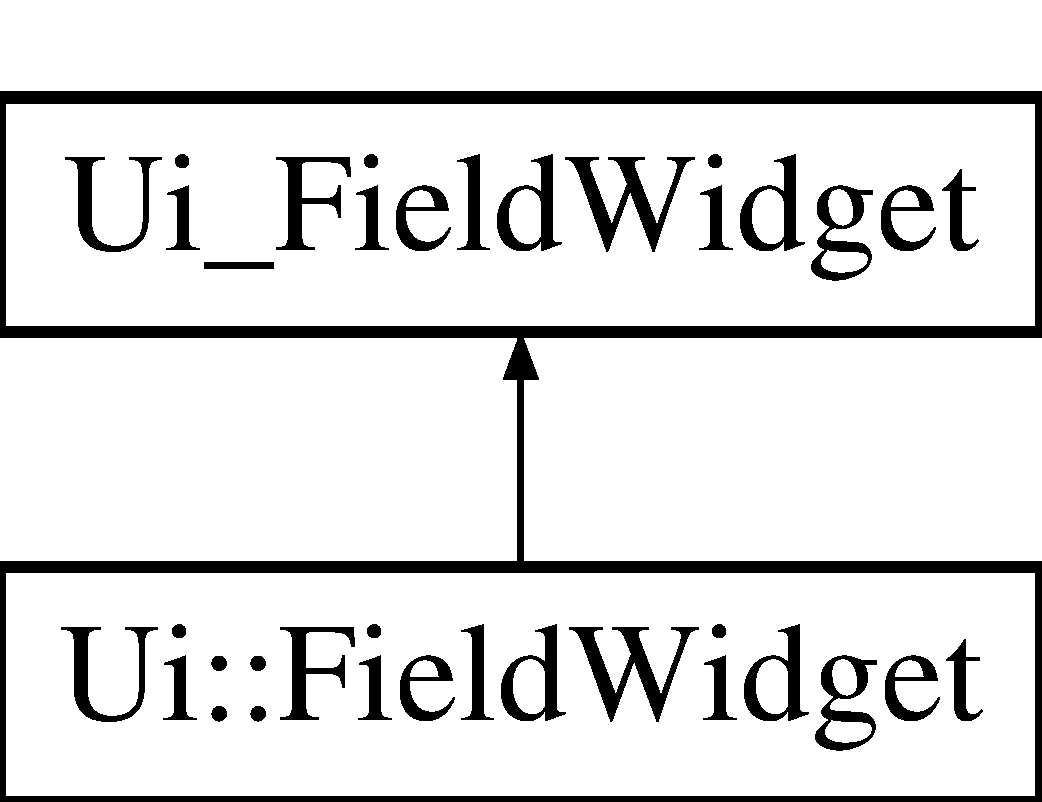
\includegraphics[height=2.000000cm]{class_ui_1_1_field_widget}
\end{center}
\end{figure}
\subsection*{Additional Inherited Members}


The documentation for this class was generated from the following file\+:\begin{DoxyCompactItemize}
\item 
ui\+\_\+fieldwidget.\+h\end{DoxyCompactItemize}

\hypertarget{class_game}{}\section{Game Class Reference}
\label{class_game}\index{Game@{Game}}
Inheritance diagram for Game\+:\begin{figure}[H]
\begin{center}
\leavevmode
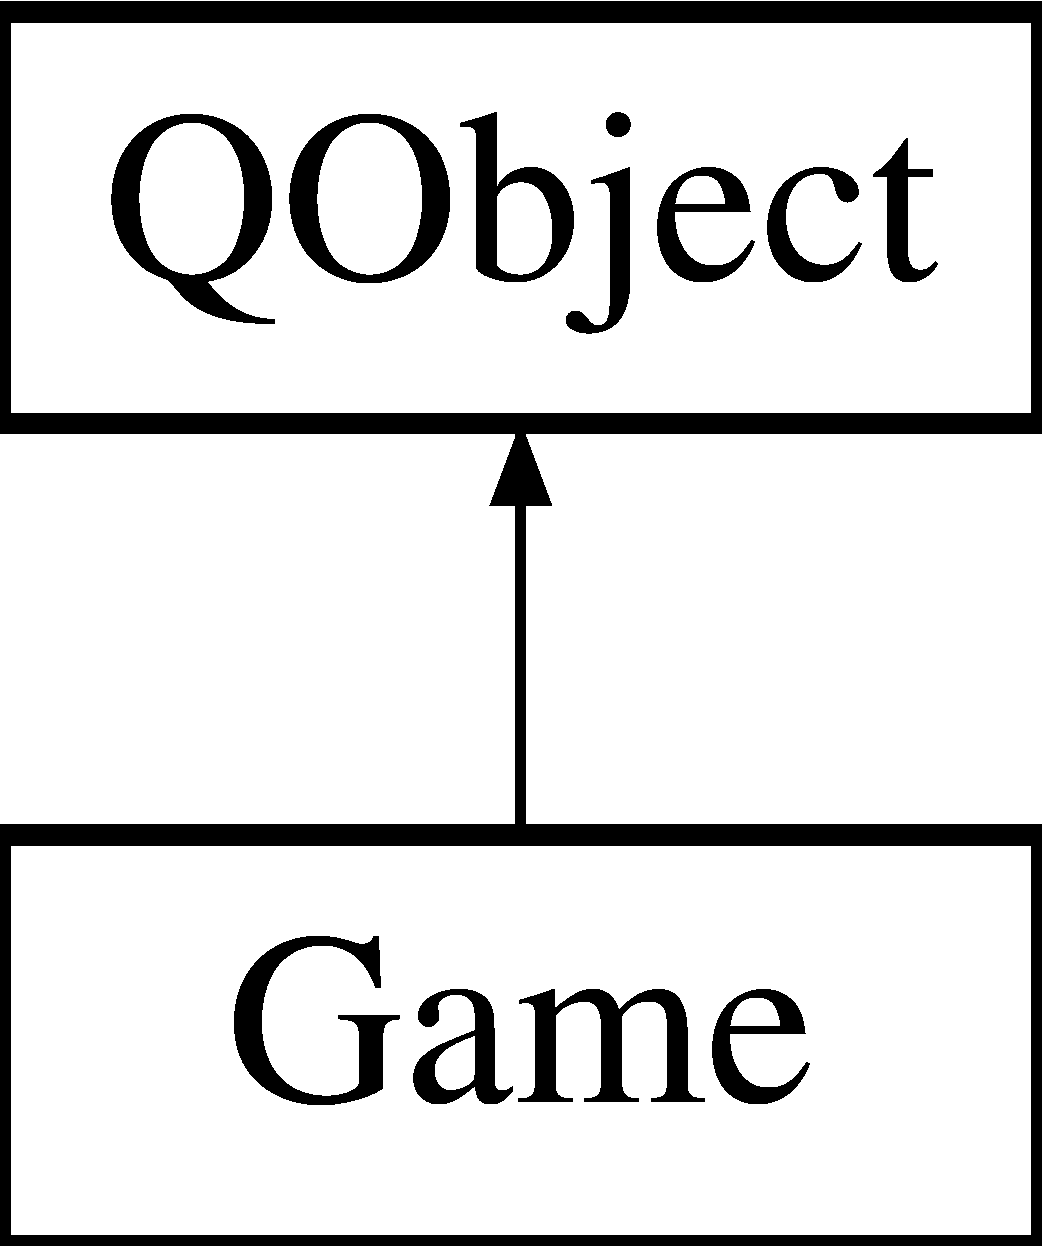
\includegraphics[height=2.000000cm]{class_game}
\end{center}
\end{figure}
\subsection*{Public Slots}
\begin{DoxyCompactItemize}
\item 
\mbox{\Hypertarget{class_game_adb6ad159b4ba797928b16e7e5910f359}\label{class_game_adb6ad159b4ba797928b16e7e5910f359}} 
void {\bfseries \+\_\+input\+Card\+\_\+} (\hyperlink{class_card}{Card} $\ast$)
\item 
\mbox{\Hypertarget{class_game_a0a7c4c6cad38634438e69afd759fc9bc}\label{class_game_a0a7c4c6cad38634438e69afd759fc9bc}} 
void {\bfseries \+\_\+input\+Card\+Set\+\_\+} (\hyperlink{class_card_set}{Card\+Set} $\ast$)
\item 
\mbox{\Hypertarget{class_game_a07db123f744de984c1f96ea8eceee69c}\label{class_game_a07db123f744de984c1f96ea8eceee69c}} 
void {\bfseries \+\_\+input\+Order\+\_\+} (int)
\item 
\mbox{\Hypertarget{class_game_a36487a0ad7c9e09889726c351a18c849}\label{class_game_a36487a0ad7c9e09889726c351a18c849}} 
void {\bfseries end\+Turn} (int, int)
\item 
\mbox{\Hypertarget{class_game_ae892651cc87c8ea057a4b157923b3de9}\label{class_game_ae892651cc87c8ea057a4b157923b3de9}} 
void {\bfseries end\+Round} (int)
\item 
\mbox{\Hypertarget{class_game_a7d88788cf4b0da39a0245d418aa6f37a}\label{class_game_a7d88788cf4b0da39a0245d418aa6f37a}} 
void {\bfseries end\+Game} ()
\item 
\mbox{\Hypertarget{class_game_ae8638ccdb0ef3bf39a6affa30aa1258f}\label{class_game_ae8638ccdb0ef3bf39a6affa30aa1258f}} 
void {\bfseries start\+Game} ()
\item 
\mbox{\Hypertarget{class_game_ac8bdb1c74e094c5fb191fd8dd33cdb1e}\label{class_game_ac8bdb1c74e094c5fb191fd8dd33cdb1e}} 
void {\bfseries start\+Round} (int, int)
\item 
\mbox{\Hypertarget{class_game_ac09956e6593c89266c705040df122372}\label{class_game_ac09956e6593c89266c705040df122372}} 
void {\bfseries start\+Turn} (int, int)
\end{DoxyCompactItemize}
\subsection*{Signals}
\begin{DoxyCompactItemize}
\item 
\mbox{\Hypertarget{class_game_af3736b24c708412dc9cfb4f8d44d8bcc}\label{class_game_af3736b24c708412dc9cfb4f8d44d8bcc}} 
void {\bfseries \+\_\+start\+Game} ()
\item 
\mbox{\Hypertarget{class_game_a0ec6b4656d13c00b185bae314e44d1ab}\label{class_game_a0ec6b4656d13c00b185bae314e44d1ab}} 
void {\bfseries \+\_\+start\+Round} (int, int)
\item 
\mbox{\Hypertarget{class_game_a2331a7e63f909db8b07c595b313d526a}\label{class_game_a2331a7e63f909db8b07c595b313d526a}} 
void {\bfseries \+\_\+start\+Turn} (int, int)
\item 
\mbox{\Hypertarget{class_game_a9510c5bdc2808d69050ef3e7ab999e62}\label{class_game_a9510c5bdc2808d69050ef3e7ab999e62}} 
void {\bfseries \+\_\+end\+Round} (int)
\item 
\mbox{\Hypertarget{class_game_a570a056019eb5328fac83381ec82e8a8}\label{class_game_a570a056019eb5328fac83381ec82e8a8}} 
void {\bfseries \+\_\+end\+Turn} (int, int)
\item 
\mbox{\Hypertarget{class_game_a0f52ae0a6a8fdd7bb6946ea962e6d6da}\label{class_game_a0f52ae0a6a8fdd7bb6946ea962e6d6da}} 
void {\bfseries \+\_\+end\+Game} ()
\item 
\mbox{\Hypertarget{class_game_afc3047129b167f5a7f39fda51d544fa5}\label{class_game_afc3047129b167f5a7f39fda51d544fa5}} 
void {\bfseries start\+Game\+\_\+} ()
\item 
\mbox{\Hypertarget{class_game_a6feae0777b3cfc5fd6f7cde33d6a901b}\label{class_game_a6feae0777b3cfc5fd6f7cde33d6a901b}} 
void {\bfseries start\+Round\+\_\+} (int, int)
\item 
\mbox{\Hypertarget{class_game_a025f44b0026e936fca4aff4ae13d2e17}\label{class_game_a025f44b0026e936fca4aff4ae13d2e17}} 
void {\bfseries start\+Turn\+\_\+} (int, int)
\item 
\mbox{\Hypertarget{class_game_a1cab6bf318963908e71508531a702641}\label{class_game_a1cab6bf318963908e71508531a702641}} 
void {\bfseries end\+Round\+\_\+} ()
\item 
\mbox{\Hypertarget{class_game_a863cdd926ca08ec8ab24dd4a4cc1a719}\label{class_game_a863cdd926ca08ec8ab24dd4a4cc1a719}} 
void {\bfseries end\+Turn\+\_\+} (int, int)
\item 
\mbox{\Hypertarget{class_game_a009d960d4a3904936242838d0ee1f288}\label{class_game_a009d960d4a3904936242838d0ee1f288}} 
void {\bfseries end\+Game\+\_\+} ()
\item 
\mbox{\Hypertarget{class_game_a68434e8fd97ea4ced1b66800f6f28cba}\label{class_game_a68434e8fd97ea4ced1b66800f6f28cba}} 
void {\bfseries \+\_\+input\+Card} (\hyperlink{class_card_set}{Card\+Set} $\ast$)
\item 
\mbox{\Hypertarget{class_game_ad05a31ab4777b0dc195a58c9451002de}\label{class_game_ad05a31ab4777b0dc195a58c9451002de}} 
void {\bfseries \+\_\+input\+Card\+Set} (list$<$ \hyperlink{class_card_set}{Card\+Set} $\ast$$>$ $\ast$)
\item 
\mbox{\Hypertarget{class_game_a9684a513c8de2ce34f918925d6db5152}\label{class_game_a9684a513c8de2ce34f918925d6db5152}} 
void {\bfseries \+\_\+input\+Order} (\hyperlink{class_card_set}{Card\+Set} $\ast$)
\item 
\mbox{\Hypertarget{class_game_a51f8b19c1fbadff3bb6110a0838f41d1}\label{class_game_a51f8b19c1fbadff3bb6110a0838f41d1}} 
void {\bfseries \+\_\+query\+Pass} ()
\item 
\mbox{\Hypertarget{class_game_a042b23c59b55a8e1bfb037d323985655}\label{class_game_a042b23c59b55a8e1bfb037d323985655}} 
void {\bfseries \+\_\+gameover} ()
\end{DoxyCompactItemize}
\subsection*{Public Member Functions}
\begin{DoxyCompactItemize}
\item 
\mbox{\Hypertarget{class_game_a1875963fc898101a29d47084aebffa28}\label{class_game_a1875963fc898101a29d47084aebffa28}} 
{\bfseries Game} (Q\+Object $\ast$parent=0)
\item 
\mbox{\Hypertarget{class_game_a3ff63bc03af3e579bada089f42d0c133}\label{class_game_a3ff63bc03af3e579bada089f42d0c133}} 
void {\bfseries \+\_\+\+\_\+init} ()
\item 
\mbox{\Hypertarget{class_game_ae5cfc450417808cdcb76cf48c8ff072a}\label{class_game_ae5cfc450417808cdcb76cf48c8ff072a}} 
void {\bfseries \+\_\+\+\_\+test} ()
\item 
\mbox{\Hypertarget{class_game_ae631dec4007607be119441ee2a8baa26}\label{class_game_ae631dec4007607be119441ee2a8baa26}} 
\hyperlink{class_card}{Card} $\ast$ {\bfseries \+\_\+\+\_\+pop\+Front\+\_\+card\+Input} ()
\item 
\mbox{\Hypertarget{class_game_ac2b080efeb6aab8aa7d176f2fa051a5e}\label{class_game_ac2b080efeb6aab8aa7d176f2fa051a5e}} 
\hyperlink{class_card_set}{Card\+Set} $\ast$ {\bfseries \+\_\+\+\_\+pop\+Front\+\_\+card\+Set\+Input} ()
\item 
\mbox{\Hypertarget{class_game_a3735b6e5a4c2c08058e748962e01413f}\label{class_game_a3735b6e5a4c2c08058e748962e01413f}} 
int {\bfseries \+\_\+\+\_\+pop\+Front\+\_\+order\+Input} ()
\end{DoxyCompactItemize}
\subsection*{Public Attributes}
\begin{DoxyCompactItemize}
\item 
\mbox{\Hypertarget{class_game_a3cae3709d3d57b9f128e3eb98c84ba32}\label{class_game_a3cae3709d3d57b9f128e3eb98c84ba32}} 
\hyperlink{class_field}{Field} $\ast$ {\bfseries field}
\item 
\mbox{\Hypertarget{class_game_a0bcdbe1720c9f053b48ca1e603d78ef3}\label{class_game_a0bcdbe1720c9f053b48ca1e603d78ef3}} 
\hyperlink{class_user_interaction}{User\+Interaction} $\ast$ {\bfseries user} \mbox{[}M\+A\+X\+\_\+\+T\+E\+A\+M\+\_\+\+N\+UM\mbox{]}
\item 
\mbox{\Hypertarget{class_game_a868bd58affa0cff32e3adb229e454bf1}\label{class_game_a868bd58affa0cff32e3adb229e454bf1}} 
Q\+String {\bfseries deckpath} \mbox{[}2\mbox{]}
\item 
\mbox{\Hypertarget{class_game_af13900cf8080e61eb5dc257653bb3928}\label{class_game_af13900cf8080e61eb5dc257653bb3928}} 
Q\+String {\bfseries card\+Dir}
\item 
\mbox{\Hypertarget{class_game_a99d07be4a79a71f986f59b09e98c5006}\label{class_game_a99d07be4a79a71f986f59b09e98c5006}} 
int {\bfseries cur\+Team}
\item 
\mbox{\Hypertarget{class_game_a9087c3cd44012a3f321bea7cac6e243c}\label{class_game_a9087c3cd44012a3f321bea7cac6e243c}} 
int {\bfseries round}
\item 
\mbox{\Hypertarget{class_game_ad3199bedc32504d5f56019289ca02b73}\label{class_game_ad3199bedc32504d5f56019289ca02b73}} 
int {\bfseries score} \mbox{[}M\+A\+X\+\_\+\+T\+E\+A\+M\+\_\+\+N\+UM\mbox{]}\mbox{[}M\+A\+X\+\_\+\+R\+O\+U\+N\+D\+\_\+\+N\+UM\mbox{]}
\item 
\mbox{\Hypertarget{class_game_ad521168cca3db47e9eb96223e13ef428}\label{class_game_ad521168cca3db47e9eb96223e13ef428}} 
int {\bfseries win\+Round} \mbox{[}M\+A\+X\+\_\+\+T\+E\+A\+M\+\_\+\+N\+UM\mbox{]}
\item 
\mbox{\Hypertarget{class_game_a1ca42dbcccd79399445577e2fed0e49f}\label{class_game_a1ca42dbcccd79399445577e2fed0e49f}} 
int {\bfseries passed} \mbox{[}M\+A\+X\+\_\+\+T\+E\+A\+M\+\_\+\+N\+UM\mbox{]}
\item 
\mbox{\Hypertarget{class_game_a00ab5d9b77844791934ee8cc1fdbd07f}\label{class_game_a00ab5d9b77844791934ee8cc1fdbd07f}} 
list$<$ \hyperlink{class_card}{Card} $\ast$ $>$ {\bfseries card\+Input}
\item 
\mbox{\Hypertarget{class_game_a9e7f61bf7e7499b41f65e1d4fac10c7b}\label{class_game_a9e7f61bf7e7499b41f65e1d4fac10c7b}} 
list$<$ \hyperlink{class_card_set}{Card\+Set} $\ast$ $>$ {\bfseries card\+Set\+Input}
\item 
\mbox{\Hypertarget{class_game_aba73af76bd69cae2248361ab83f41c06}\label{class_game_aba73af76bd69cae2248361ab83f41c06}} 
list$<$ int $>$ {\bfseries order\+Input}
\end{DoxyCompactItemize}


The documentation for this class was generated from the following files\+:\begin{DoxyCompactItemize}
\item 
game.\+h\item 
game.\+cpp\end{DoxyCompactItemize}

\hypertarget{class_input_dialog}{}\section{Input\+Dialog Class Reference}
\label{class_input_dialog}\index{Input\+Dialog@{Input\+Dialog}}
Inheritance diagram for Input\+Dialog\+:\begin{figure}[H]
\begin{center}
\leavevmode
\includegraphics[height=2.000000cm]{class_input_dialog}
\end{center}
\end{figure}
\subsection*{Public Slots}
\begin{DoxyCompactItemize}
\item 
\mbox{\Hypertarget{class_input_dialog_a9350aaf68e3c3d3879ffa92b0a0abeca}\label{class_input_dialog_a9350aaf68e3c3d3879ffa92b0a0abeca}} 
void {\bfseries submit\+\_\+clicked} ()
\item 
\mbox{\Hypertarget{class_input_dialog_a6cc8e60359a166d15c48a6e7543c72fc}\label{class_input_dialog_a6cc8e60359a166d15c48a6e7543c72fc}} 
void {\bfseries update\+Data} (S\+I\+\_\+\+String)
\end{DoxyCompactItemize}
\subsection*{Public Member Functions}
\begin{DoxyCompactItemize}
\item 
\mbox{\Hypertarget{class_input_dialog_a348ae820e563de9aed5077a2bbaf15b5}\label{class_input_dialog_a348ae820e563de9aed5077a2bbaf15b5}} 
{\bfseries Input\+Dialog} (Q\+Widget $\ast$parent=0)
\end{DoxyCompactItemize}


The documentation for this class was generated from the following files\+:\begin{DoxyCompactItemize}
\item 
inputdialog.\+h\item 
inputdialog.\+cpp\end{DoxyCompactItemize}

\input{class_ui_1_1_main_window}
\hypertarget{class_main_window}{}\section{Main\+Window Class Reference}
\label{class_main_window}\index{Main\+Window@{Main\+Window}}
Inheritance diagram for Main\+Window\+:\begin{figure}[H]
\begin{center}
\leavevmode
\includegraphics[height=2.000000cm]{class_main_window}
\end{center}
\end{figure}
\subsection*{Public Slots}
\begin{DoxyCompactItemize}
\item 
\mbox{\Hypertarget{class_main_window_a90e37d8ff96b5c5aef941aaa93f523f6}\label{class_main_window_a90e37d8ff96b5c5aef941aaa93f523f6}} 
void {\bfseries slot\+\_\+deckbuilder} ()
\item 
\mbox{\Hypertarget{class_main_window_af01ad1b1153fd076e35909c09d46087b}\label{class_main_window_af01ad1b1153fd076e35909c09d46087b}} 
void {\bfseries slot\+\_\+startgame} ()
\end{DoxyCompactItemize}
\subsection*{Public Member Functions}
\begin{DoxyCompactItemize}
\item 
\mbox{\Hypertarget{class_main_window_a8b244be8b7b7db1b08de2a2acb9409db}\label{class_main_window_a8b244be8b7b7db1b08de2a2acb9409db}} 
{\bfseries Main\+Window} (Q\+Widget $\ast$parent=0)
\end{DoxyCompactItemize}


The documentation for this class was generated from the following files\+:\begin{DoxyCompactItemize}
\item 
mainwindow.\+h\item 
mainwindow.\+cpp\end{DoxyCompactItemize}

\hypertarget{class_select_dialog}{}\section{Select\+Dialog Class Reference}
\label{class_select_dialog}\index{Select\+Dialog@{Select\+Dialog}}
Inheritance diagram for Select\+Dialog\+:\begin{figure}[H]
\begin{center}
\leavevmode
\includegraphics[height=2.000000cm]{class_select_dialog}
\end{center}
\end{figure}
\subsection*{Public Member Functions}
\begin{DoxyCompactItemize}
\item 
\mbox{\Hypertarget{class_select_dialog_a5c77144fb8eadc97861eaa6643f7941a}\label{class_select_dialog_a5c77144fb8eadc97861eaa6643f7941a}} 
{\bfseries Select\+Dialog} (Q\+Widget $\ast$parent=0)
\end{DoxyCompactItemize}


The documentation for this class was generated from the following files\+:\begin{DoxyCompactItemize}
\item 
selectdialog.\+h\item 
selectdialog.\+cpp\end{DoxyCompactItemize}

\hypertarget{class_ui_1_1_select_dialog}{}\section{Ui\+:\+:Select\+Dialog Class Reference}
\label{class_ui_1_1_select_dialog}\index{Ui\+::\+Select\+Dialog@{Ui\+::\+Select\+Dialog}}
Inheritance diagram for Ui\+:\+:Select\+Dialog\+:\begin{figure}[H]
\begin{center}
\leavevmode
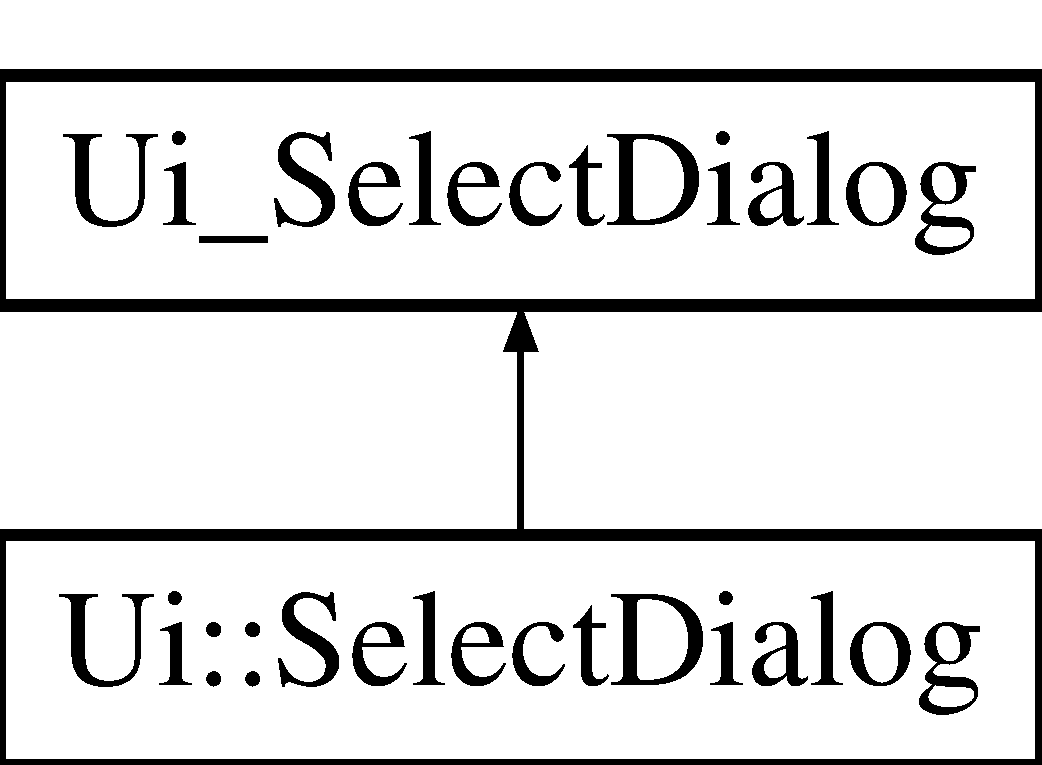
\includegraphics[height=2.000000cm]{class_ui_1_1_select_dialog}
\end{center}
\end{figure}
\subsection*{Additional Inherited Members}


The documentation for this class was generated from the following file\+:\begin{DoxyCompactItemize}
\item 
ui\+\_\+selectdialog.\+h\end{DoxyCompactItemize}

\hypertarget{class_s_i___object}{}\section{S\+I\+\_\+\+Object Class Reference}
\label{class_s_i___object}\index{S\+I\+\_\+\+Object@{S\+I\+\_\+\+Object}}
Inheritance diagram for S\+I\+\_\+\+Object\+:\begin{figure}[H]
\begin{center}
\leavevmode
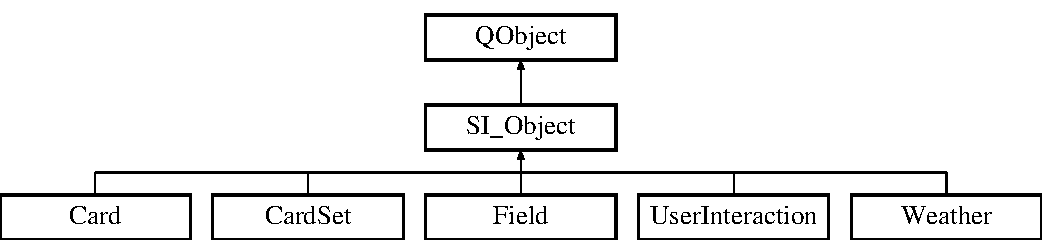
\includegraphics[height=3.000000cm]{class_s_i___object}
\end{center}
\end{figure}
\subsection*{Public Slots}
\begin{DoxyCompactItemize}
\item 
\mbox{\Hypertarget{class_s_i___object_a9c997aa5f9bc1670872e7a59b3dddd93}\label{class_s_i___object_a9c997aa5f9bc1670872e7a59b3dddd93}} 
virtual void {\bfseries \+\_\+adjust\+Property\+\_\+} (S\+I\+\_\+\+String, S\+I\+\_\+\+String, S\+I\+\_\+\+String, \hyperlink{class_s_i___object}{S\+I\+\_\+\+Object} $\ast$, S\+I\+\_\+\+String)
\item 
\mbox{\Hypertarget{class_s_i___object_afa18ebaf13b5ca5de7382ca0950b2016}\label{class_s_i___object_afa18ebaf13b5ca5de7382ca0950b2016}} 
void {\bfseries set\+Property} (const S\+I\+\_\+\+String \&, const S\+I\+\_\+\+String \&)
\end{DoxyCompactItemize}
\subsection*{Signals}
\begin{DoxyCompactItemize}
\item 
\mbox{\Hypertarget{class_s_i___object_acead0d8f20e267fc9c40cf865c975769}\label{class_s_i___object_acead0d8f20e267fc9c40cf865c975769}} 
void {\bfseries adjust\+Property\+\_\+} (S\+I\+\_\+\+String, S\+I\+\_\+\+String, S\+I\+\_\+\+String, \hyperlink{class_s_i___object}{S\+I\+\_\+\+Object} $\ast$, S\+I\+\_\+\+String)
\end{DoxyCompactItemize}
\subsection*{Public Member Functions}
\begin{DoxyCompactItemize}
\item 
\mbox{\Hypertarget{class_s_i___object_a6ec637849a43d4d6eb9cd41f649cc1ec}\label{class_s_i___object_a6ec637849a43d4d6eb9cd41f649cc1ec}} 
{\bfseries S\+I\+\_\+\+Object} (Q\+Object $\ast$parent=0)
\item 
\mbox{\Hypertarget{class_s_i___object_a9ec2d414baa9b92d0fd6a3404f2ee2d7}\label{class_s_i___object_a9ec2d414baa9b92d0fd6a3404f2ee2d7}} 
{\bfseries S\+I\+\_\+\+Object} (const \hyperlink{class_s_i___object}{S\+I\+\_\+\+Object} \&)
\item 
\mbox{\Hypertarget{class_s_i___object_a68431e1d8f5383b8519cf5a451737cb8}\label{class_s_i___object_a68431e1d8f5383b8519cf5a451737cb8}} 
S\+I\+\_\+\+String {\bfseries get\+Property} (const S\+I\+\_\+\+String \&) const
\item 
\mbox{\Hypertarget{class_s_i___object_af617bfe0cbc89aa2a62ceeb2b34233d3}\label{class_s_i___object_af617bfe0cbc89aa2a62ceeb2b34233d3}} 
Q\+Map$<$ S\+I\+\_\+\+String, S\+I\+\_\+\+String $>$\+::iterator {\bfseries get\+Begin} ()
\item 
\mbox{\Hypertarget{class_s_i___object_ac2a9abad4b05bfc1800a915bcbe63025}\label{class_s_i___object_ac2a9abad4b05bfc1800a915bcbe63025}} 
Q\+Map$<$ S\+I\+\_\+\+String, S\+I\+\_\+\+String $>$\+::iterator {\bfseries get\+End} ()
\item 
\mbox{\Hypertarget{class_s_i___object_a2464e6bfc480a09dca8ad7d610660f90}\label{class_s_i___object_a2464e6bfc480a09dca8ad7d610660f90}} 
void {\bfseries \+\_\+\+\_\+\+\_\+print\+\_\+properties} ()
\end{DoxyCompactItemize}
\subsection*{Public Attributes}
\begin{DoxyCompactItemize}
\item 
\mbox{\Hypertarget{class_s_i___object_a32f0018fcbae8593d45f84cf06f33f8e}\label{class_s_i___object_a32f0018fcbae8593d45f84cf06f33f8e}} 
Q\+Map$<$ S\+I\+\_\+\+String, S\+I\+\_\+\+String $>$ {\bfseries properties}
\end{DoxyCompactItemize}


The documentation for this class was generated from the following files\+:\begin{DoxyCompactItemize}
\item 
si\+\_\+object.\+h\item 
si\+\_\+object.\+cpp\end{DoxyCompactItemize}

\hypertarget{class_ui___battle_dialog}{}\section{Ui\+\_\+\+Battle\+Dialog Class Reference}
\label{class_ui___battle_dialog}\index{Ui\+\_\+\+Battle\+Dialog@{Ui\+\_\+\+Battle\+Dialog}}
Inheritance diagram for Ui\+\_\+\+Battle\+Dialog\+:\begin{figure}[H]
\begin{center}
\leavevmode
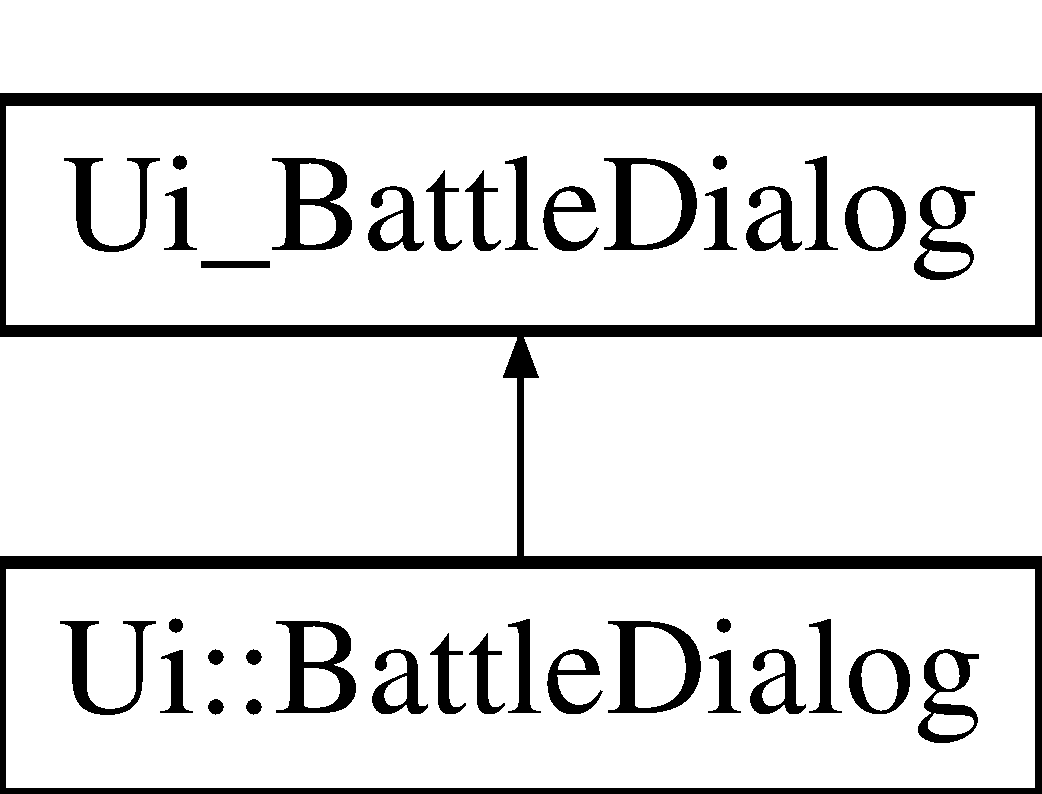
\includegraphics[height=2.000000cm]{class_ui___battle_dialog}
\end{center}
\end{figure}
\subsection*{Public Member Functions}
\begin{DoxyCompactItemize}
\item 
\mbox{\Hypertarget{class_ui___battle_dialog_a47d2abc875c2881b4889707e3d30701d}\label{class_ui___battle_dialog_a47d2abc875c2881b4889707e3d30701d}} 
void {\bfseries setup\+Ui} (Q\+Dialog $\ast$\hyperlink{class_battle_dialog}{Battle\+Dialog})
\item 
\mbox{\Hypertarget{class_ui___battle_dialog_a63d360f0f0a813f1c9119208281e7fb1}\label{class_ui___battle_dialog_a63d360f0f0a813f1c9119208281e7fb1}} 
void {\bfseries retranslate\+Ui} (Q\+Dialog $\ast$\hyperlink{class_battle_dialog}{Battle\+Dialog})
\end{DoxyCompactItemize}


The documentation for this class was generated from the following file\+:\begin{DoxyCompactItemize}
\item 
ui\+\_\+battledialog.\+h\end{DoxyCompactItemize}

\hypertarget{class_ui___card_set_widget}{}\section{Ui\+\_\+\+Card\+Set\+Widget Class Reference}
\label{class_ui___card_set_widget}\index{Ui\+\_\+\+Card\+Set\+Widget@{Ui\+\_\+\+Card\+Set\+Widget}}
Inheritance diagram for Ui\+\_\+\+Card\+Set\+Widget\+:\begin{figure}[H]
\begin{center}
\leavevmode
\includegraphics[height=2.000000cm]{class_ui___card_set_widget}
\end{center}
\end{figure}
\subsection*{Public Member Functions}
\begin{DoxyCompactItemize}
\item 
\mbox{\Hypertarget{class_ui___card_set_widget_a09c5c8e9182b53ce9aa36fc8d90c24e8}\label{class_ui___card_set_widget_a09c5c8e9182b53ce9aa36fc8d90c24e8}} 
void {\bfseries setup\+Ui} (Q\+Widget $\ast$\hyperlink{class_card_set_widget}{Card\+Set\+Widget})
\item 
\mbox{\Hypertarget{class_ui___card_set_widget_a25c48a39c22d590848875135c01b9e8b}\label{class_ui___card_set_widget_a25c48a39c22d590848875135c01b9e8b}} 
void {\bfseries retranslate\+Ui} (Q\+Widget $\ast$\hyperlink{class_card_set_widget}{Card\+Set\+Widget})
\end{DoxyCompactItemize}


The documentation for this class was generated from the following file\+:\begin{DoxyCompactItemize}
\item 
ui\+\_\+cardsetwidget.\+h\end{DoxyCompactItemize}

\hypertarget{class_ui___card_widget}{}\section{Ui\+\_\+\+Card\+Widget Class Reference}
\label{class_ui___card_widget}\index{Ui\+\_\+\+Card\+Widget@{Ui\+\_\+\+Card\+Widget}}
Inheritance diagram for Ui\+\_\+\+Card\+Widget\+:\begin{figure}[H]
\begin{center}
\leavevmode
\includegraphics[height=2.000000cm]{class_ui___card_widget}
\end{center}
\end{figure}
\subsection*{Public Member Functions}
\begin{DoxyCompactItemize}
\item 
\mbox{\Hypertarget{class_ui___card_widget_aa6f73f9fd9070f98ed108783ede6f538}\label{class_ui___card_widget_aa6f73f9fd9070f98ed108783ede6f538}} 
void {\bfseries setup\+Ui} (Q\+Widget $\ast$\hyperlink{class_card_widget}{Card\+Widget})
\item 
\mbox{\Hypertarget{class_ui___card_widget_a182f67da8cdd1cf87c97f9e01ad4bef7}\label{class_ui___card_widget_a182f67da8cdd1cf87c97f9e01ad4bef7}} 
void {\bfseries retranslate\+Ui} (Q\+Widget $\ast$\hyperlink{class_card_widget}{Card\+Widget})
\end{DoxyCompactItemize}


The documentation for this class was generated from the following file\+:\begin{DoxyCompactItemize}
\item 
ui\+\_\+cardwidget.\+h\end{DoxyCompactItemize}

\hypertarget{class_ui___field_widget}{}\section{Ui\+\_\+\+Field\+Widget Class Reference}
\label{class_ui___field_widget}\index{Ui\+\_\+\+Field\+Widget@{Ui\+\_\+\+Field\+Widget}}
Inheritance diagram for Ui\+\_\+\+Field\+Widget\+:\begin{figure}[H]
\begin{center}
\leavevmode
\includegraphics[height=2.000000cm]{class_ui___field_widget}
\end{center}
\end{figure}
\subsection*{Public Member Functions}
\begin{DoxyCompactItemize}
\item 
\mbox{\Hypertarget{class_ui___field_widget_abadaef52ee8016abce85f45454b2fa8e}\label{class_ui___field_widget_abadaef52ee8016abce85f45454b2fa8e}} 
void {\bfseries setup\+Ui} (Q\+Widget $\ast$\hyperlink{class_field_widget}{Field\+Widget})
\item 
\mbox{\Hypertarget{class_ui___field_widget_ad0cb82ccef5035b6e5f2ccb21db96be7}\label{class_ui___field_widget_ad0cb82ccef5035b6e5f2ccb21db96be7}} 
void {\bfseries retranslate\+Ui} (Q\+Widget $\ast$\hyperlink{class_field_widget}{Field\+Widget})
\end{DoxyCompactItemize}


The documentation for this class was generated from the following file\+:\begin{DoxyCompactItemize}
\item 
ui\+\_\+fieldwidget.\+h\end{DoxyCompactItemize}

\input{class_ui___main_window}
\hypertarget{class_ui___select_dialog}{}\section{Ui\+\_\+\+Select\+Dialog Class Reference}
\label{class_ui___select_dialog}\index{Ui\+\_\+\+Select\+Dialog@{Ui\+\_\+\+Select\+Dialog}}
Inheritance diagram for Ui\+\_\+\+Select\+Dialog\+:\begin{figure}[H]
\begin{center}
\leavevmode
\includegraphics[height=2.000000cm]{class_ui___select_dialog}
\end{center}
\end{figure}
\subsection*{Public Member Functions}
\begin{DoxyCompactItemize}
\item 
\mbox{\Hypertarget{class_ui___select_dialog_abdb56e4111bc4c1a3145811084647974}\label{class_ui___select_dialog_abdb56e4111bc4c1a3145811084647974}} 
void {\bfseries setup\+Ui} (Q\+Dialog $\ast$\hyperlink{class_select_dialog}{Select\+Dialog})
\item 
\mbox{\Hypertarget{class_ui___select_dialog_ae7dbc45a4f195c5b3f05abaac2c9f237}\label{class_ui___select_dialog_ae7dbc45a4f195c5b3f05abaac2c9f237}} 
void {\bfseries retranslate\+Ui} (Q\+Dialog $\ast$\hyperlink{class_select_dialog}{Select\+Dialog})
\end{DoxyCompactItemize}


The documentation for this class was generated from the following file\+:\begin{DoxyCompactItemize}
\item 
ui\+\_\+selectdialog.\+h\end{DoxyCompactItemize}

\hypertarget{class_user_interaction}{}\section{User\+Interaction Class Reference}
\label{class_user_interaction}\index{User\+Interaction@{User\+Interaction}}
Inheritance diagram for User\+Interaction\+:\begin{figure}[H]
\begin{center}
\leavevmode
\includegraphics[height=3.000000cm]{class_user_interaction}
\end{center}
\end{figure}
\subsection*{Public Slots}
\begin{DoxyCompactItemize}
\item 
\mbox{\Hypertarget{class_user_interaction_a19c4330dde326f5593946abf8f7cd213}\label{class_user_interaction_a19c4330dde326f5593946abf8f7cd213}} 
void {\bfseries input\+Card} (\hyperlink{class_card_set}{Card\+Set} $\ast$)
\item 
\mbox{\Hypertarget{class_user_interaction_a65714650c645b9c1865500702b553b7e}\label{class_user_interaction_a65714650c645b9c1865500702b553b7e}} 
void {\bfseries input\+Card\+Set} (list$<$ \hyperlink{class_card_set}{Card\+Set} $\ast$$>$ $\ast$)
\item 
\mbox{\Hypertarget{class_user_interaction_a3d7c9ea75ca204150e2d2a3aacdda72a}\label{class_user_interaction_a3d7c9ea75ca204150e2d2a3aacdda72a}} 
void {\bfseries input\+Order} (\hyperlink{class_card_set}{Card\+Set} $\ast$)
\item 
\mbox{\Hypertarget{class_user_interaction_ab7bce422790b17da78f8cdb45b928013}\label{class_user_interaction_ab7bce422790b17da78f8cdb45b928013}} 
void {\bfseries query\+Pass} ()
\item 
\mbox{\Hypertarget{class_user_interaction_a5c4d87eabeb266804c9241b65c198ccc}\label{class_user_interaction_a5c4d87eabeb266804c9241b65c198ccc}} 
int {\bfseries query\+Bin} (S\+I\+\_\+\+String)
\end{DoxyCompactItemize}
\subsection*{Signals}
\begin{DoxyCompactItemize}
\item 
\mbox{\Hypertarget{class_user_interaction_ab1c91337e7453bfee5feff257aa67059}\label{class_user_interaction_ab1c91337e7453bfee5feff257aa67059}} 
void {\bfseries input\+Card\+\_\+} (\hyperlink{class_card}{Card} $\ast$)
\item 
\mbox{\Hypertarget{class_user_interaction_a251514670bae830664958d369de19508}\label{class_user_interaction_a251514670bae830664958d369de19508}} 
void {\bfseries input\+Card\+Set\+\_\+} (\hyperlink{class_card_set}{Card\+Set} $\ast$)
\item 
\mbox{\Hypertarget{class_user_interaction_ad5b22af9c1b6fa7e6545d58f7321076a}\label{class_user_interaction_ad5b22af9c1b6fa7e6545d58f7321076a}} 
void {\bfseries input\+Order\+\_\+} (int)
\item 
\mbox{\Hypertarget{class_user_interaction_a34b7c252ebf9ba7eb90856859b5d06fc}\label{class_user_interaction_a34b7c252ebf9ba7eb90856859b5d06fc}} 
void {\bfseries \+\_\+pass} (int)
\end{DoxyCompactItemize}
\subsection*{Public Member Functions}
\begin{DoxyCompactItemize}
\item 
\mbox{\Hypertarget{class_user_interaction_a4aeac47b93a4faf9bfc28e1a9c82ae31}\label{class_user_interaction_a4aeac47b93a4faf9bfc28e1a9c82ae31}} 
{\bfseries User\+Interaction} (int team, \hyperlink{class_game}{Game} $\ast$pgame, Q\+Object $\ast$parent=0)
\item 
\mbox{\Hypertarget{class_user_interaction_a649516d648a3c6e06cf66b676ec57e0f}\label{class_user_interaction_a649516d648a3c6e06cf66b676ec57e0f}} 
\hyperlink{class_card}{Card} $\ast$ {\bfseries \+\_\+\+\_\+input\+Card} (\hyperlink{class_card_set}{Card\+Set} $\ast$)
\item 
\mbox{\Hypertarget{class_user_interaction_a0c2e1a09df22e3980ddc62dd9af81441}\label{class_user_interaction_a0c2e1a09df22e3980ddc62dd9af81441}} 
\hyperlink{class_card_set}{Card\+Set} $\ast$ {\bfseries \+\_\+\+\_\+input\+Card\+Set} (list$<$ \hyperlink{class_card_set}{Card\+Set} $\ast$$>$ $\ast$)
\item 
\mbox{\Hypertarget{class_user_interaction_a5a7ad04bed1d90079e9995b5e3d43640}\label{class_user_interaction_a5a7ad04bed1d90079e9995b5e3d43640}} 
int {\bfseries \+\_\+\+\_\+input\+Order} (\hyperlink{class_card_set}{Card\+Set} $\ast$)
\item 
\mbox{\Hypertarget{class_user_interaction_a3e439e45021b61aadaeac96141591c94}\label{class_user_interaction_a3e439e45021b61aadaeac96141591c94}} 
int {\bfseries \+\_\+\+\_\+input\+Place} (\hyperlink{class_card}{Card} $\ast$, \hyperlink{class_card_set}{Card\+Set} $\ast$\&, int \&)
\item 
\mbox{\Hypertarget{class_user_interaction_a14cbffbf423eaa5c5ca9d12e2a0d3bc1}\label{class_user_interaction_a14cbffbf423eaa5c5ca9d12e2a0d3bc1}} 
S\+I\+\_\+\+String {\bfseries get\+Team} ()
\end{DoxyCompactItemize}
\subsection*{Public Attributes}
\begin{DoxyCompactItemize}
\item 
\mbox{\Hypertarget{class_user_interaction_a6788061b735de7f1a86180b2fa4982c1}\label{class_user_interaction_a6788061b735de7f1a86180b2fa4982c1}} 
\hyperlink{class_game}{Game} $\ast$ {\bfseries game}
\end{DoxyCompactItemize}


The documentation for this class was generated from the following files\+:\begin{DoxyCompactItemize}
\item 
userinteraction.\+h\item 
userinteraction.\+cpp\end{DoxyCompactItemize}

\hypertarget{class_weather}{}\section{Weather Class Reference}
\label{class_weather}\index{Weather@{Weather}}
Inheritance diagram for Weather\+:\begin{figure}[H]
\begin{center}
\leavevmode
\includegraphics[height=4.000000cm]{class_weather}
\end{center}
\end{figure}
\subsection*{Public Slots}
\begin{DoxyCompactItemize}
\item 
\mbox{\Hypertarget{class_weather_a71873b46a578c3056113ce306de8d34e}\label{class_weather_a71873b46a578c3056113ce306de8d34e}} 
virtual void {\bfseries \+\_\+start\+Turn\+\_\+} (int, int)
\end{DoxyCompactItemize}
\subsection*{Public Member Functions}
\begin{DoxyCompactItemize}
\item 
\mbox{\Hypertarget{class_weather_a1aa40de6a7c41ad78d2d64cbf9b43ba0}\label{class_weather_a1aa40de6a7c41ad78d2d64cbf9b43ba0}} 
{\bfseries Weather} (Q\+Object $\ast$parent=0)
\item 
\mbox{\Hypertarget{class_weather_aa2bcf44c4341922b806aaa4b5839003c}\label{class_weather_aa2bcf44c4341922b806aaa4b5839003c}} 
{\bfseries Weather} (const \hyperlink{class_weather}{Weather} \&)
\item 
\mbox{\Hypertarget{class_weather_a565411dad19031111d17b4a89770491a}\label{class_weather_a565411dad19031111d17b4a89770491a}} 
void {\bfseries \+\_\+\+\_\+do\+Connect} ()
\item 
\mbox{\Hypertarget{class_weather_a7bcdf5987eee6f28e8e3ea4bf6558602}\label{class_weather_a7bcdf5987eee6f28e8e3ea4bf6558602}} 
void {\bfseries set\+To\+Row} (\hyperlink{class_card_set}{Card\+Set} $\ast$)
\item 
\mbox{\Hypertarget{class_weather_a3b5578263e2c356e25dd49dd3582ac17}\label{class_weather_a3b5578263e2c356e25dd49dd3582ac17}} 
void {\bfseries remove\+From\+Row} ()
\item 
\mbox{\Hypertarget{class_weather_af777d66f1dfa7587345e67c41d2d4bf2}\label{class_weather_af777d66f1dfa7587345e67c41d2d4bf2}} 
void {\bfseries \+\_\+\+\_\+init} ()
\end{DoxyCompactItemize}
\subsection*{Static Public Member Functions}
\begin{DoxyCompactItemize}
\item 
\mbox{\Hypertarget{class_weather_a53a322e5f96d16a913ac9e4fe963dbf6}\label{class_weather_a53a322e5f96d16a913ac9e4fe963dbf6}} 
static \hyperlink{class_weather}{Weather} $\ast$ {\bfseries factory} (\hyperlink{class_game}{Game} $\ast$, const S\+I\+\_\+\+String \&)
\end{DoxyCompactItemize}
\subsection*{Public Attributes}
\begin{DoxyCompactItemize}
\item 
\mbox{\Hypertarget{class_weather_a0c9c6e62a821128bad912cd65abf8773}\label{class_weather_a0c9c6e62a821128bad912cd65abf8773}} 
\hyperlink{class_card_set}{Card\+Set} $\ast$ {\bfseries row}
\item 
\mbox{\Hypertarget{class_weather_ae5780910b2272707d0af962f9612fb3d}\label{class_weather_ae5780910b2272707d0af962f9612fb3d}} 
\hyperlink{class_game}{Game} $\ast$ {\bfseries game}
\item 
\mbox{\Hypertarget{class_weather_ad71c0e943d232dddb6195d70d0039442}\label{class_weather_ad71c0e943d232dddb6195d70d0039442}} 
int {\bfseries id}
\item 
\mbox{\Hypertarget{class_weather_a4392e83007a52d1a33f56ccb58a52d06}\label{class_weather_a4392e83007a52d1a33f56ccb58a52d06}} 
int {\bfseries add\+Damege}
\end{DoxyCompactItemize}
\subsection*{Additional Inherited Members}


The documentation for this class was generated from the following files\+:\begin{DoxyCompactItemize}
\item 
weather.\+h\item 
weather.\+cpp\end{DoxyCompactItemize}

%--- End generated contents ---

% Index
\backmatter
\newpage
\phantomsection
\clearemptydoublepage
\addcontentsline{toc}{chapter}{Index}
\printindex

\end{document}
